%%%%%%%%%%%%%%%%%%%%%%%%%%%%%%%%%%%%%%%%%%%%%%%%%%%%%%%%%%%%%%%%%%%%%%%%%%%%%%%%%
%                                                                               %
% Cette version repart de 03_Draft\appendix\appendix_figures_tablesV1-short.tex %
%                                                                               %
%%%%%%%%%%%%%%%%%%%%%%%%%%%%%%%%%%%%%%%%%%%%%%%%%%%%%%%%%%%%%%%%%%%%%%%%%%%%%%%%%


\subsection{Figures}


\begin{figure}[h!] \centering
	\caption{LE Sample, baseline characteristics \label{fig:desc:LEquali}}
	\begin{subfigure}[b]{\textwidth}		
	\caption[]{\small Sector, NACE A10 (estimation sample vs.\ Panel DADS) \label{fig:desc:LEsec}}
		\centering
		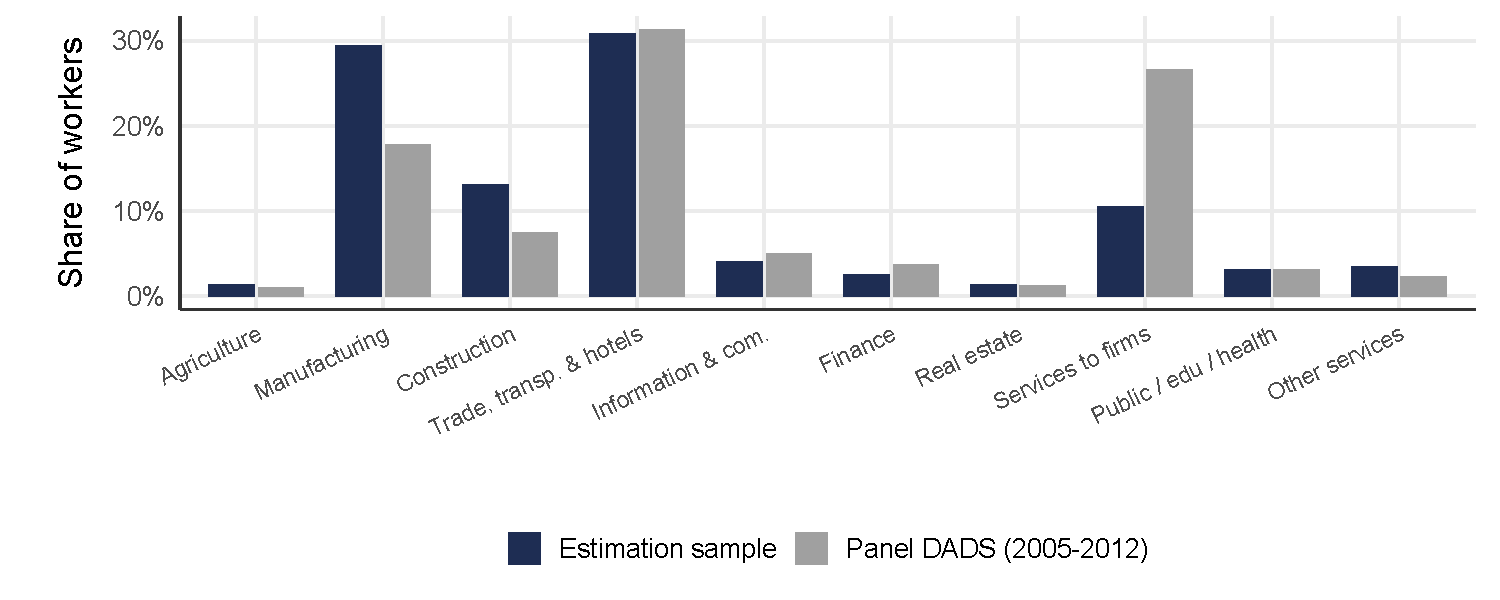
\includegraphics[width=0.69\linewidth, trim={0cm 0cm 0cm 0cm}, clip=true,max width=\linewidth]{figures/02_descriptive_figures/figure_A1_a_le_sectors.pdf}
	\end{subfigure}

	\begin{subfigure}[b]{\textwidth}
	\caption[]{\small Occupation \label{fig:desc:LEocc}}
		\centering
		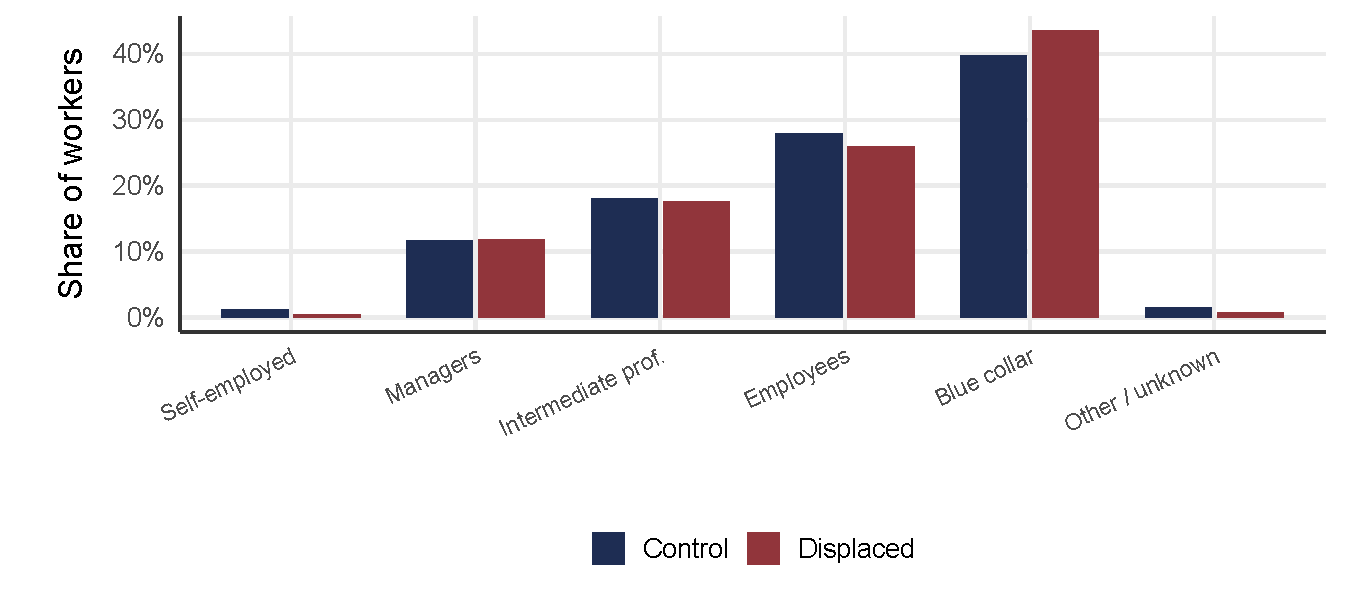
\includegraphics[scale=0.46, trim={0cm 0cm 0cm 0cm}, clip=true,max width=\linewidth]{figures/02_descriptive_figures/figure_A1_b_le_occupations.pdf}
	\end{subfigure}

	\begin{subfigure}[b]{\textwidth}
	\caption[]{\small Educational attainment \label{fig:desc:LEdip}}
		\centering
		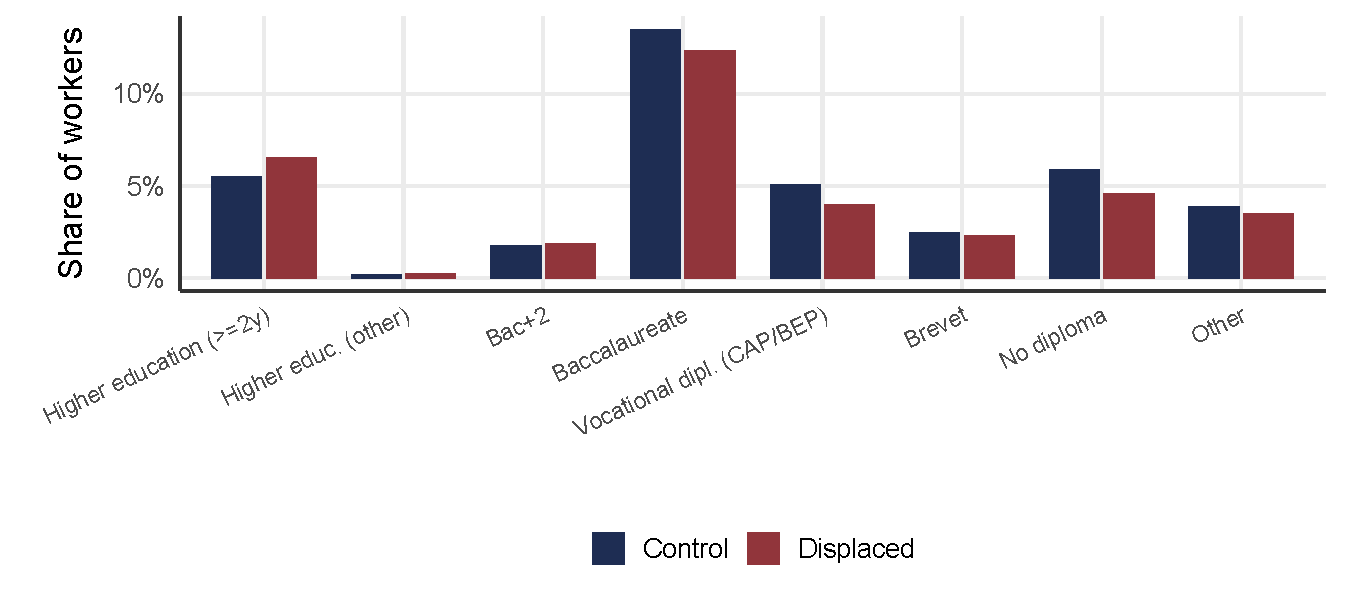
\includegraphics[scale=0.46, trim={0cm 0cm 0cm 0cm}, clip=true,max width=\linewidth]{figures/02_descriptive_figures/figure_A1_c_le_education.pdf}
	\end{subfigure}

	\floatfoot{\footnotesize{\textsc{Notes}: This figure presents descriptive statistics about the sample of 20,897 individuals displaced for economic reasons (LE) \textcolor{orange}{[21,132]} and their respective matched controls. Data is observed at $t^D-1$. Panel (a) reports the distribution of workers across NACE A10 sectors for our \emph{estimation sample} (controls only) and---for reference---the population of private-sector workers in the DADS panel over 2005--2012. We display the control group only because sector is a matching variable, so the LE-displaced and control-group distributions coincide at $t^D-1$ by construction; controls measured at $t^D-1$ are therefore an accurate description of the sectoral composition of the matched estimation sample. The third bar (Panel DADS) allows the reader to gauge how representative our estimation sample is of the broader French private-sector workforce. The ``Public / education / health'' bin (NAF~84--88) does not include employees of the central administration as our DADS sample covers only private-law contracts, so workers in this bin are employed under private-law contracts in para-public organizations such as \emph{établissements publics à caractère industriel et commercial} (EPIC), the social-security system, and private clinics, schools, and social-work non-profits operating in publicly-funded sectors. Panels (b) and (c) display the distribution of workers across occupations and educational attainment. Educational attainment is only observed for a sub-sample. These two variables were not used in the matching algorithm. In both cases, the sample appears to be balanced across treatment and controls.}}
\end{figure}


\begin{figure}[h!] \centering
	\caption{Displacement Effects in Level: Earnings, Employment and Hours} \label{fig:aveffect_emp_earn}
	%\begin{subfigure}[b]{.6\textwidth}
	%\centering
	%\caption[]{\small LE: Wage Losses} \label{fig:event_sbr}
	%\includegraphics[scale=0.3,max width=\linewidth]{03_Draft/graphs/event_sbr}
	%\end{subfigure}
	%%        \vskip
	\begin{subfigure}[b]{.49\textwidth}
		\centering
		\caption[]{\small Annual Earnings (in level) \label{fig:event_sbr}} 	
		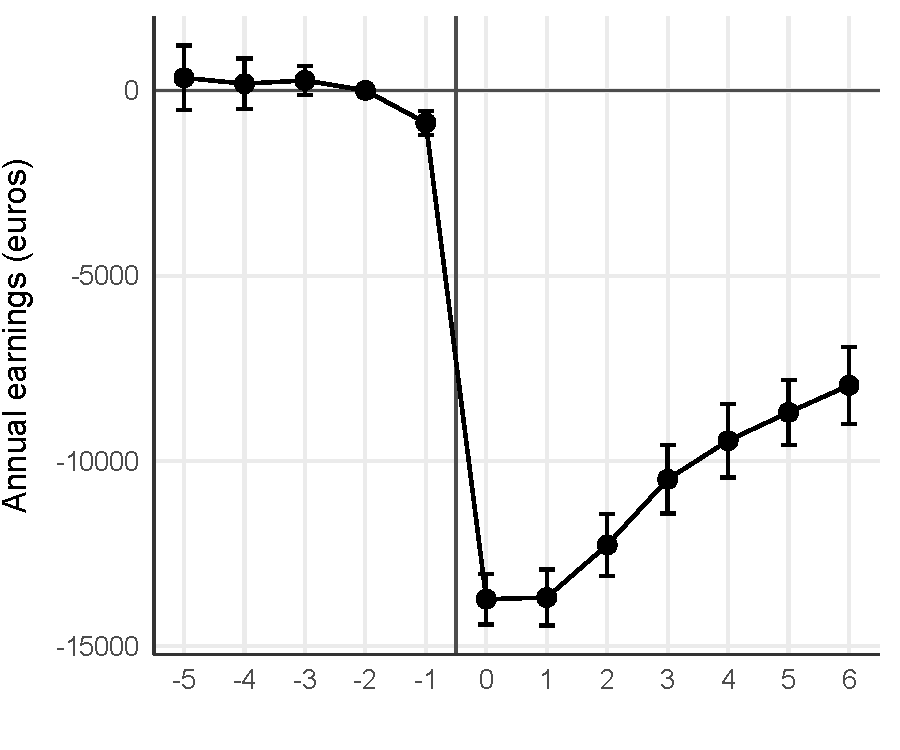
\includegraphics[scale=0.49,max width=\linewidth]{figures/01_event_figures/figure_A2_a_earnings.pdf}
	\end{subfigure}
	\begin{subfigure}[b]{.49\textwidth}
		\centering
		\caption[]{\small Employment Probability \label{fig:event_emp}} 
		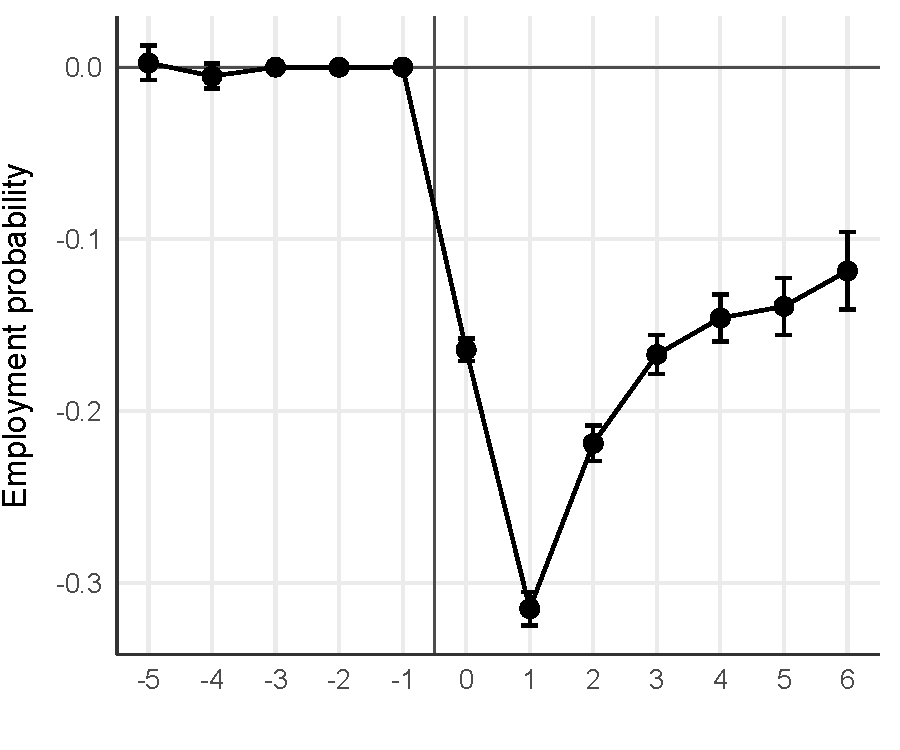
\includegraphics[scale=0.49,max width=\linewidth]{figures/01_event_figures/figure_A2_b_employment.pdf}
	\end{subfigure}
	%\vskip
	\begin{subfigure}[b]{.49\textwidth}
		\centering
		\caption[]{\small Hours Worked  \label{fig:event_hours}} 
		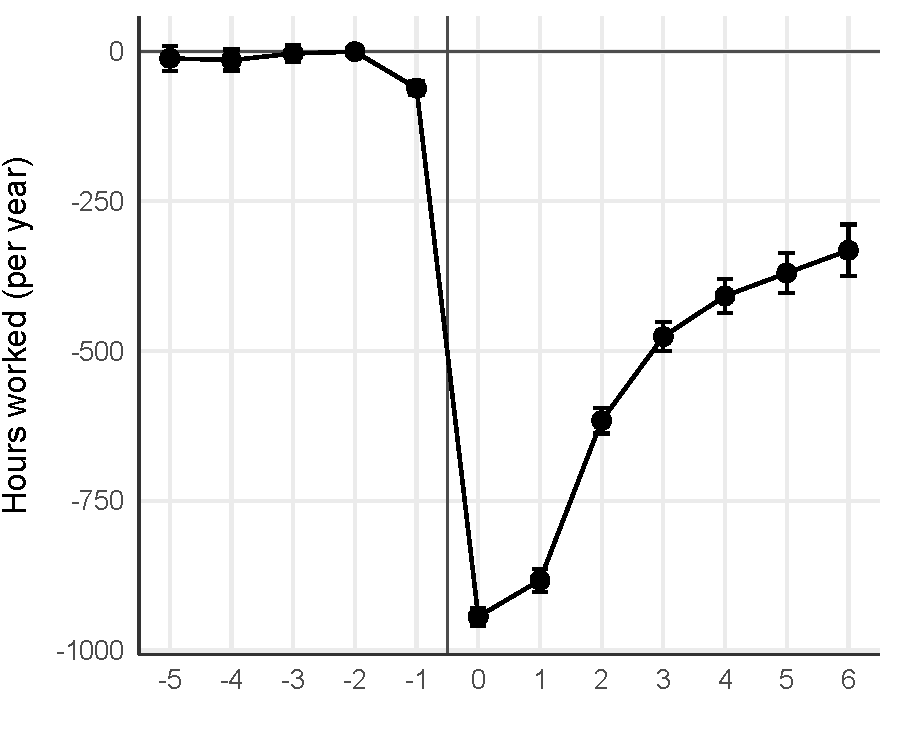
\includegraphics[scale=0.49,max width=\linewidth]{figures/01_event_figures/figure_A2_c_hours.pdf}
	\end{subfigure}
	%\begin{subfigure}[b]{.49\textwidth}
	%	\centering
	%	\caption[]{\small Hourly Wage \label{fig:event_hwr}} 
	%	\includegraphics[scale=0.49,max width=\linewidth]{figures-2026/event_lnsbrhour_Log.pdf}
	%\end{subfigure}
	
	\floatfoot{\footnotesize{\textsc{Notes}: This figure reports event-study estimates of the cost of job displacement for a sample of workers dismissed for economic reasons (LE) ---see equation (\ref{eq:main_estimating_equation}) and associated text for more details on the specification. \textbf{Samples}: The sample contains 20{,}897 individuals laid-off for economic reasons and their matched controls. All three panels use the full estimation sample; non-employed workers are assigned earnings and hours of zero. \textbf{Definition of the outcomes:} Table \ref{apptab:definitions} summarizes variables' definition. \textbf{Additional information}: Appendix Table \ref{apptab:evstudy_worker_outcomes} provides more details. For brevity, effect on hours is only displayed when using log. \textbf{Standard errors}: robust standard errors clustered at the worker-level; displayed confidence intervals at the 99\% level. }}
\end{figure}


\begin{figure}[h!]\caption{Wage decomposition on the LE sample restricted to firms with at least 10 employees}
\label{fig:wage_decomposition_size10}
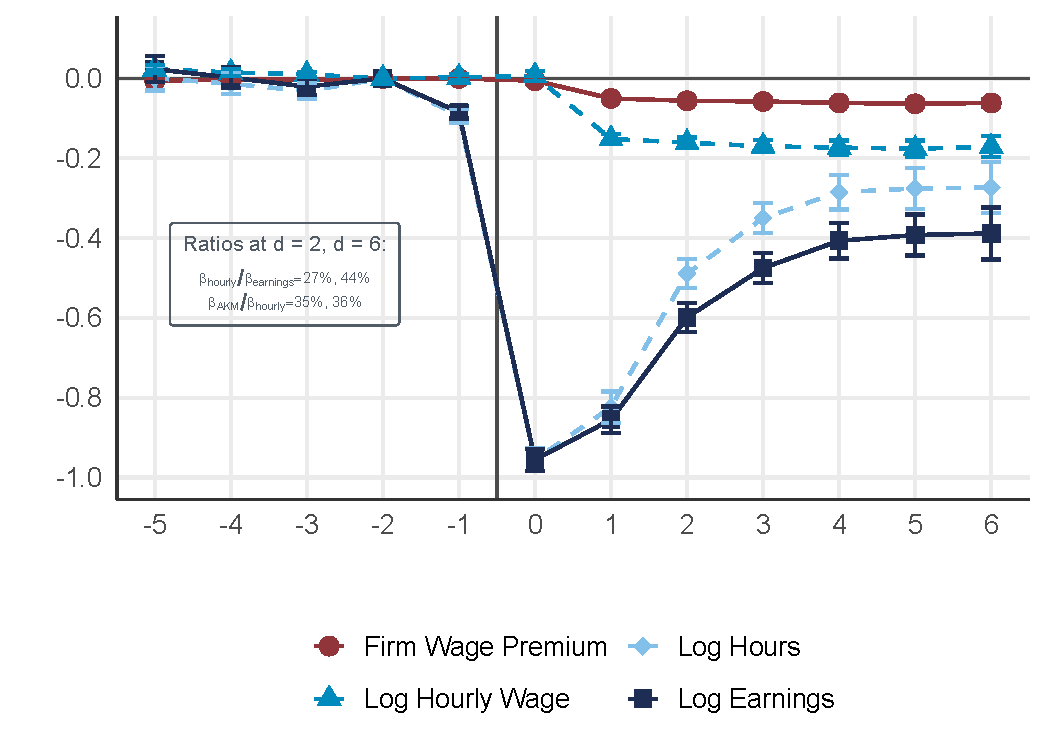
\includegraphics[width=\linewidth, trim={0cm 0cm 0.1cm 0cm}, clip,max width=\linewidth]{figures/01_event_figures/figure_A3_le_size10_wage_decomposition.pdf}
\par\medskip
\floatfoot{\footnotesize\textsc{Notes}: This figure reproduces Figure~\ref{fig:fe_current_event} of the paper (wage decomposition for the LE sample) on the subset of workers displaced from firms with at least $10$ employees prior to the event. Coefficients and ratios are very close to the baseline reported in Figure~\ref{fig:fe_current_event}, indicating that the patterns we document are not driven by displacements from very small firms.}
\end{figure}


\begin{figure}[h!]\caption{Wage decomposition on the LE sample, with unrestricted AKM (no exclusion of LE/MLO trajectories)}\label{fig:paper_R_wage_decomposition_god2}
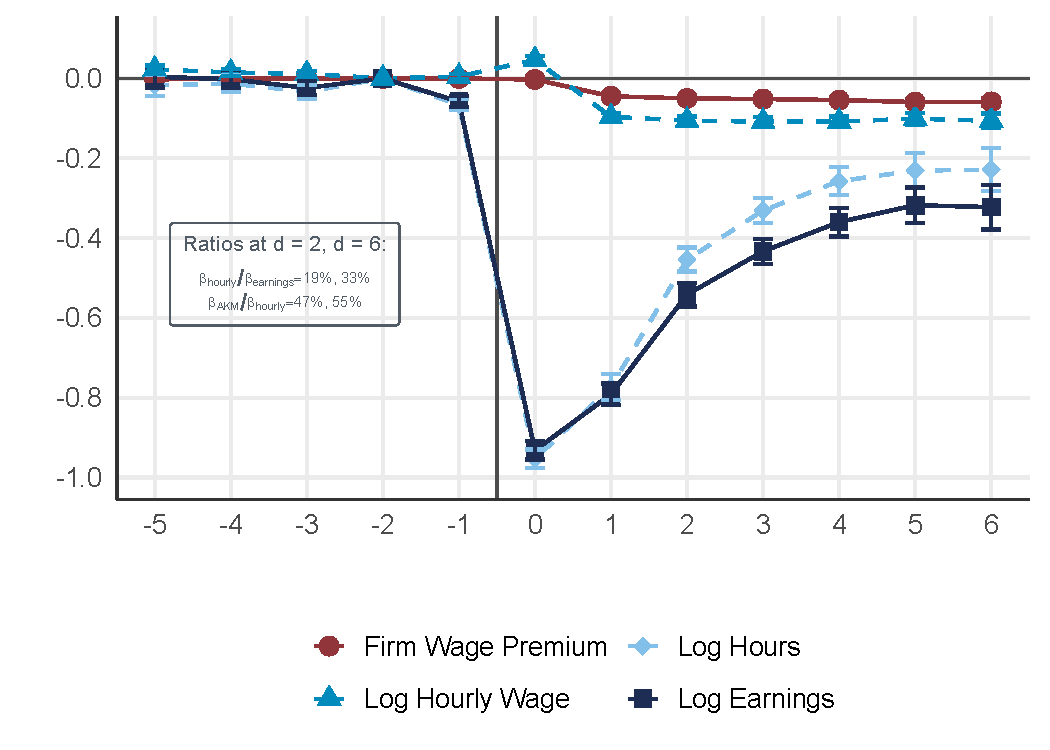
\includegraphics[width=\linewidth, trim={0cm 0cm 0.1cm 0cm}, clip,max width=\linewidth]{figures/01_event_figures/figure_A4_le_unrestricted_akm.pdf}
\par\medskip
\floatfoot{\footnotesize\textsc{Notes}: This figure reports the wage decomposition for the LE sample, using the unrestricted AKM, which does not exclude any worker, i.e. without correcting for contamination. Compared to the results in Figure~\ref{fig:fe_current_event}, the share of the hourly-wage scar attributable to the firm premium drop is larger by about $15$--$20$ percentage points under the unrestricted AKM at all post-displacement horizons. The difference reflects the bias introduced by displaced workers' post-layoff wage trajectories on the firm fixed effects of firing firms.
}
\end{figure}


% Added in the R2 revision (Referee 3, point 3): robustness of the premium loss to the AKM estimation window.
\begin{figure}[h!]\caption{Loss in firm wage premium by AKM estimation window (LE sample)}\label{fig:akm_windows}
\centering
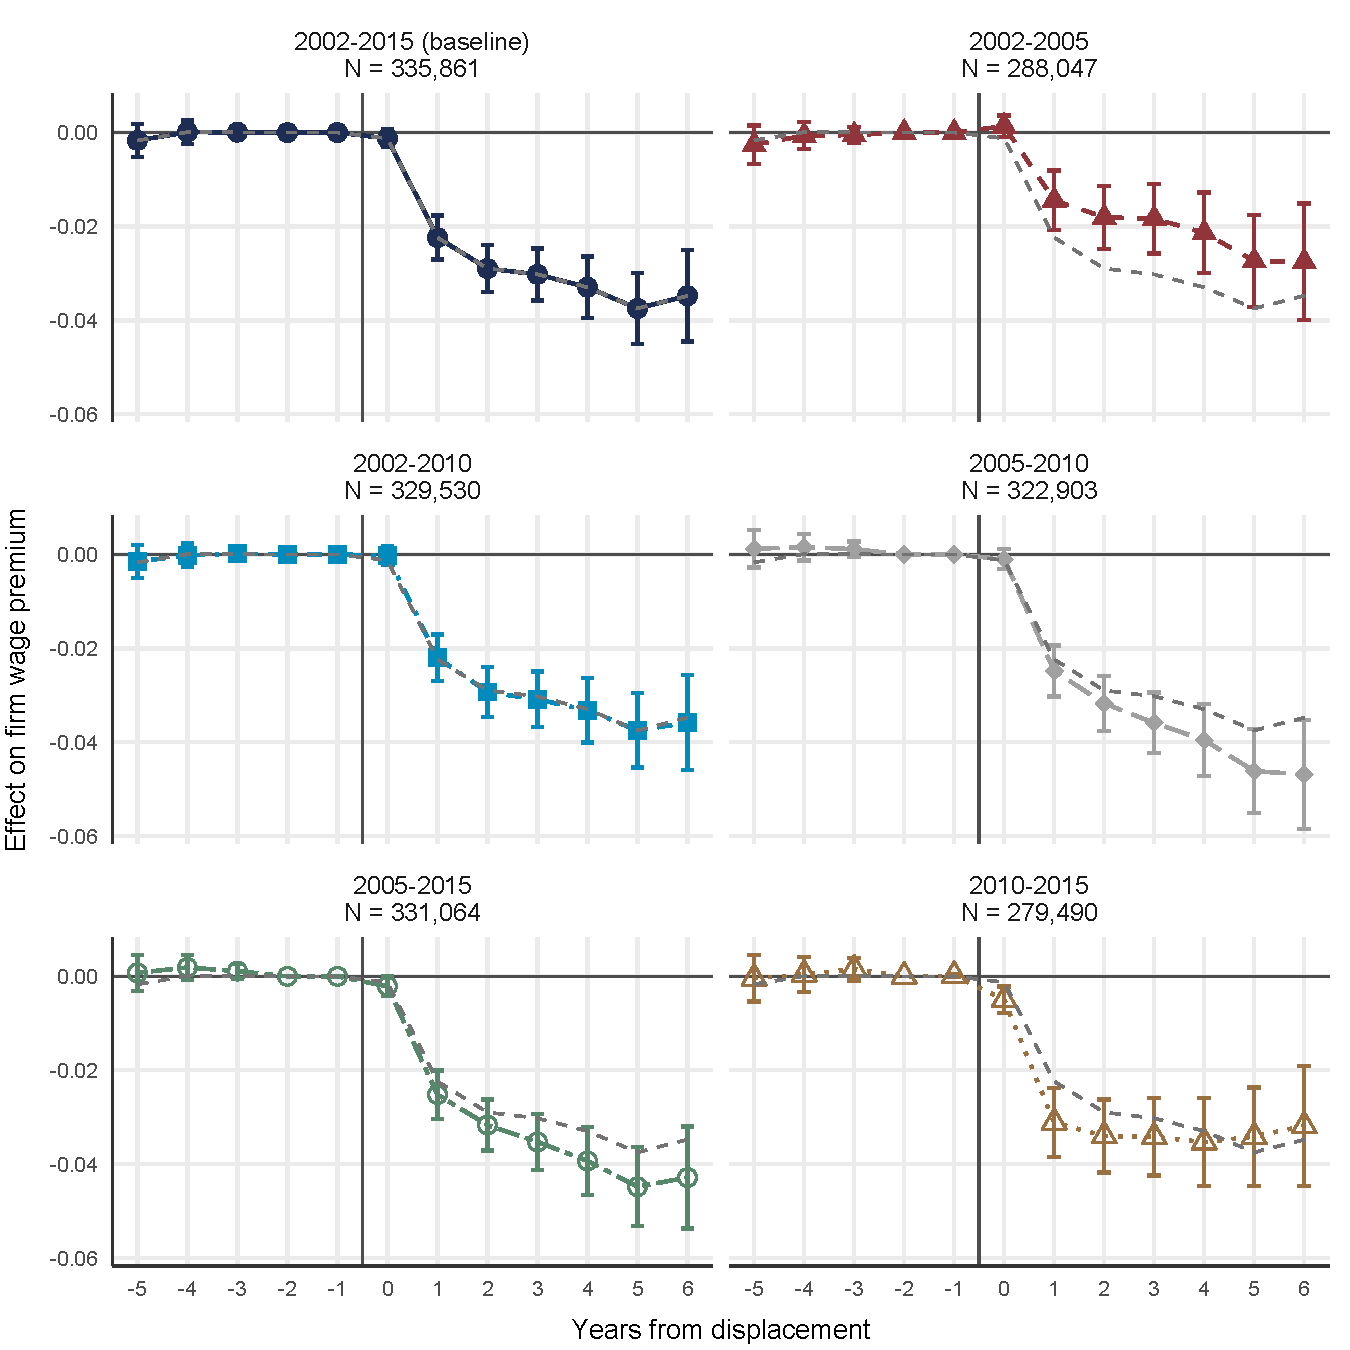
\includegraphics[width=0.95\linewidth,height=0.7\textheight,keepaspectratio]{figures/03_akm_periods/figure_A5_akm_estimation_windows.pdf}
\par\medskip
\floatfoot{\footnotesize\textsc{Notes}: Event-study estimates of the effect of job displacement on the firm wage premium of the current employer (equation \ref{eq:main_estimating_equation}), for the LE sample. In each panel, the AKM firm fixed effects are estimated over the window indicated in the title; the top-left panel (2002--2015) is the baseline of Figure \ref{fig:fe_current_event}, and is reproduced as a dashed grey line in the other panels. $N$ is the number of worker-year observations; it varies across windows because the set of firms with an estimated premium changes with the window. $t^D-2$ is the reference period. Standard errors are clustered at the worker level.}
\end{figure}


\begin{figure}[h!] \begin{center}
		\caption{Decomposition of the cost of job displacement: Mass-layoff (MLO) sample} \label{fig:fe_current_event_mlo_pretrends}
		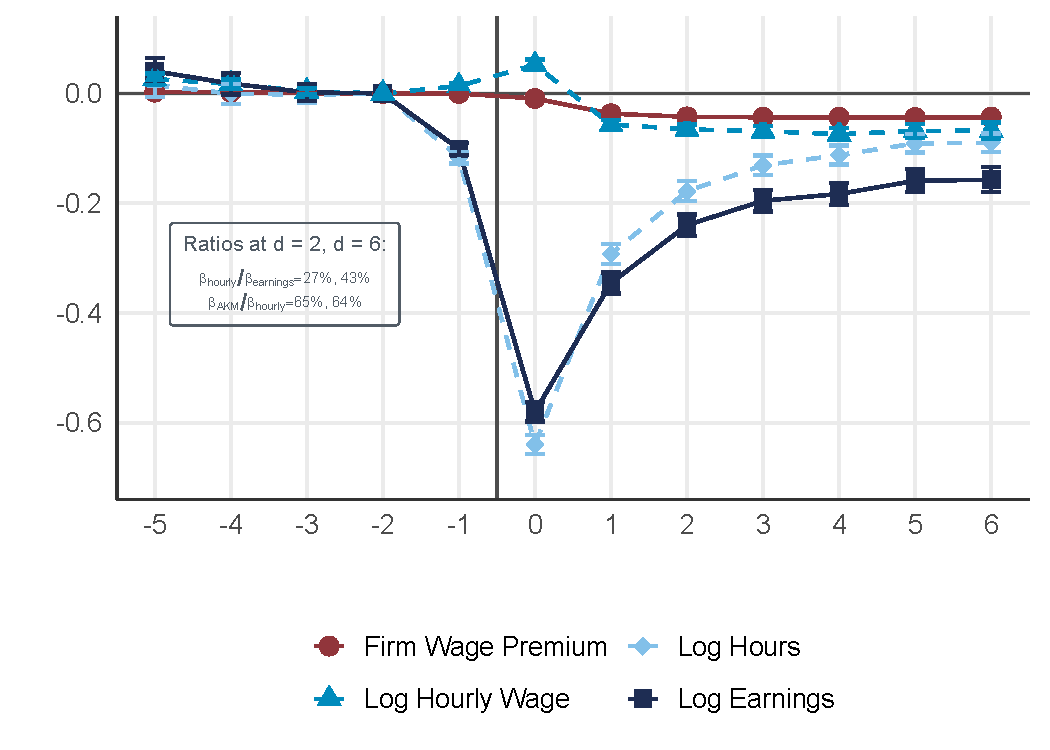
\includegraphics[width=\linewidth, trim={0cm 0cm 0.1cm 0cm}, clip,max width=\linewidth]{figures/01_event_figures/figure_A6_mlo_baseline_wage_decomposition.pdf} \\
		\floatfoot{\footnotesize{\textsc{Notes}: This figure reports event-study estimates of the effect of job displacement on log hourly wage, log hours, log earnings and firm-specific wage premium for a sample of workers displaced in a mass layoff (MLO30). It is the analogue of Figure~\ref{fig:fe_current_event} for the MLO30 sample---see equation (\ref{eq:main_estimating_equation}) and associated text for more details on the specification. \textbf{Sample}: The sample contains 17,949 individuals displaced in a mass layoff \textcolor{orange}{[17,946]} and as many controls; the regressions on log hourly wage and firm wage premium are restricted to person-distance cells with non-missing post-displacement hourly wage. Details on the construction of the sample are provided in Appendix~\ref{appsec:mlo_details}. \textbf{Outcomes}: Table~\ref{apptab:definitions} summarizes variables' definition. Wage premia are estimated, following the AKM framework, as firm-fixed effects in a two-way regression of log-hourly wage on firm and worker fixed effects---see Section~\ref{sec:data:firm:premium} for more details. \textbf{Additional information}: Table~\ref{apptab:evstudy_worker_outcomes_mlo} provides more details. \textbf{Standard errors}: robust standard errors clustered at the worker-level; displayed confidence intervals at the 99\% level.}}

\end{center} \end{figure}




\begin{figure}[h!] \centering
	\caption{Productivity, labor share and firm wage premium of current employers, MLO sample \label{fig:prod_et_al_MLO}}
	\begin{subfigure}[b]{.49\textwidth}
		\centering
		\caption[]{\small Productivity} \label{fig:prod_res_mlo}
		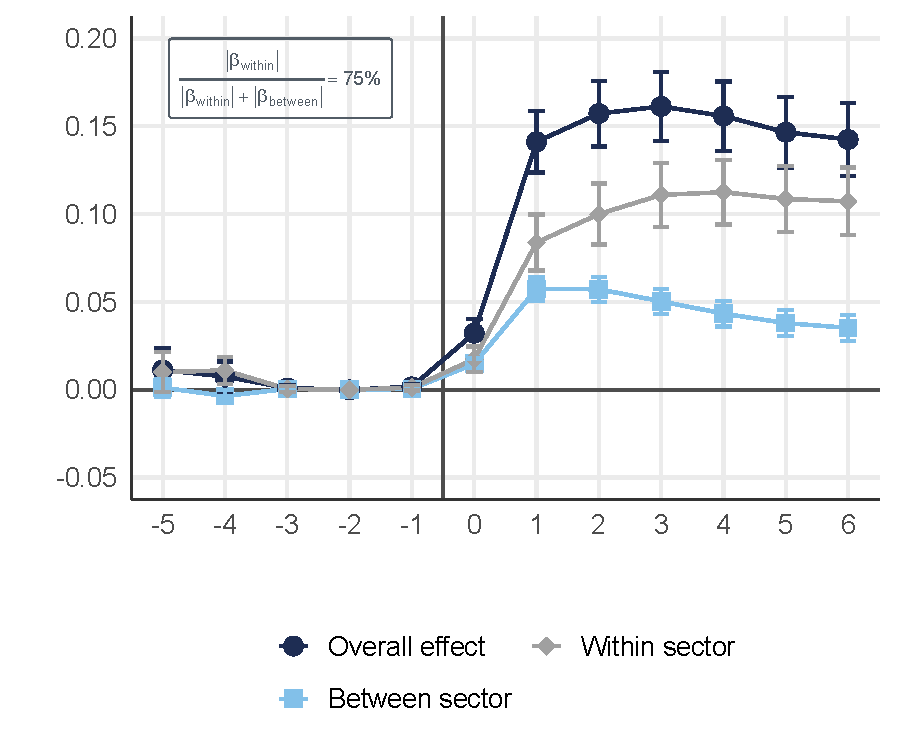
\includegraphics[scale=0.49,max width=\linewidth]{figures/01_event_figures/figure_A7_a_baseline_productivity.pdf}
	\end{subfigure}
	\begin{subfigure}[b]{.49\textwidth}
		\centering
		\caption[]{\small Labor share of value-added} \label{fig:ln_Lshare_mlo}
		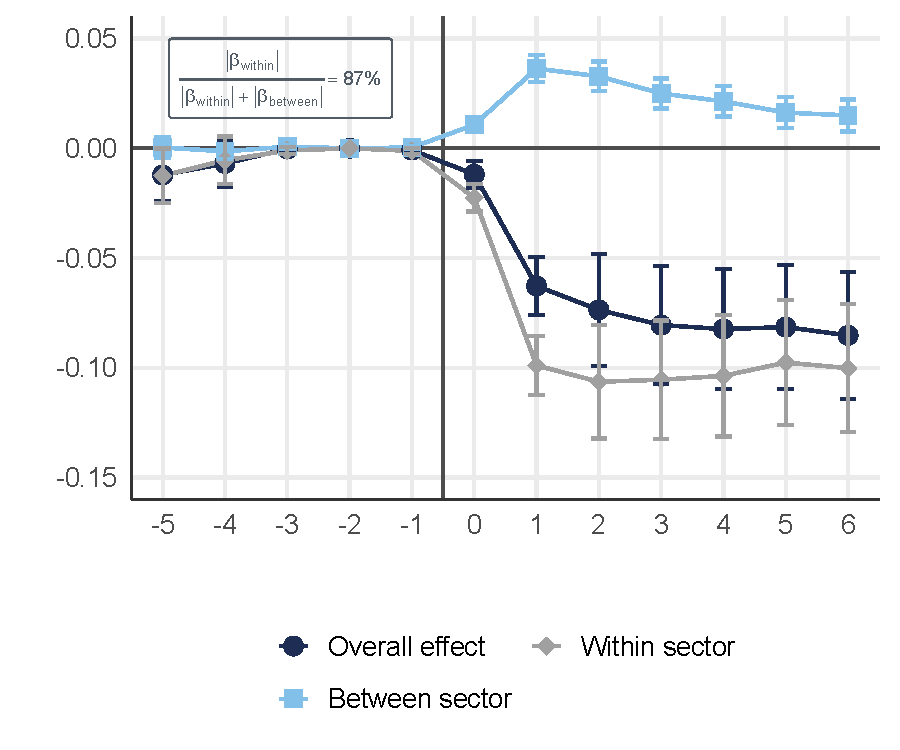
\includegraphics[scale=0.49,max width=\linewidth]{figures/01_event_figures/figure_A7_b_baseline_labor_share.pdf}
	\end{subfigure}

	\begin{subfigure}[b]{.49\textwidth}
		\caption{Firm Wage Premium} \label{fig:firm_fe_mlo}
		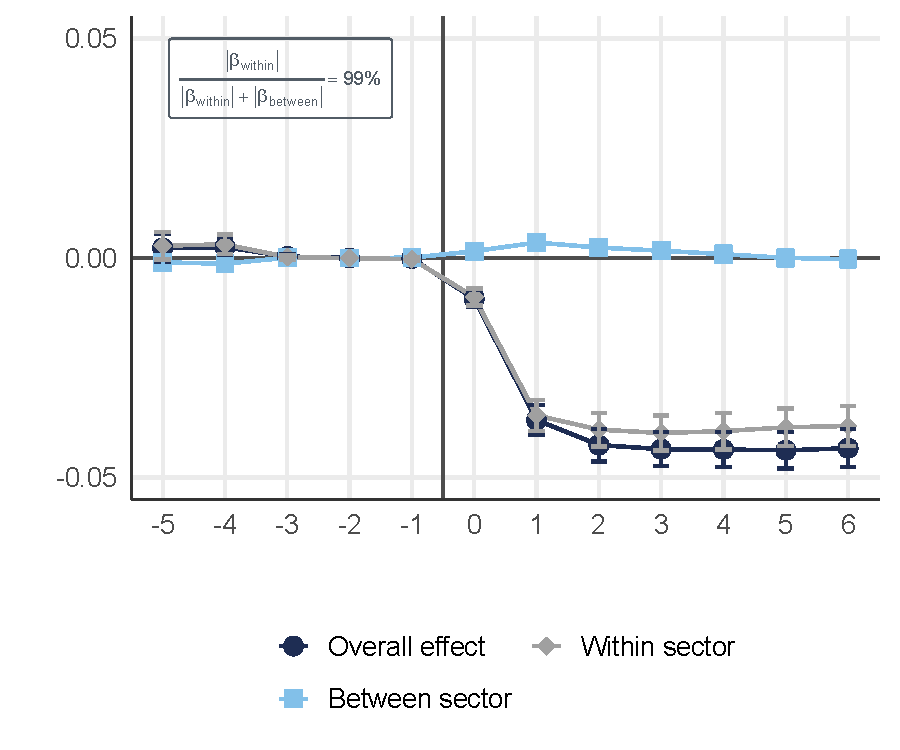
\includegraphics[width=\linewidth,max width=\linewidth]{figures/01_event_figures/figure_A7_c_baseline_firm_premium.pdf}
	\end{subfigure}

	\floatfoot{\footnotesize{\textsc{Notes}: This figure reports event-study estimates of the effect of job displacement on the reallocation of workers towards firms with varying levels of productivity, labor share, and AKM firm wage premium, for the MLO30 sample. It is the analogue of Figure~\ref{fig:ln_apl_ls} for workers displaced in a mass layoff. Coefficients are obtained by estimating the specification of equation \ref{eq:main_estimating_equation} where the dependent variable is sequentially productivity, labor share, and firm wage premium. \textbf{Sample}: The sample contains 17,949 individuals displaced in a mass layoff \textcolor{orange}{[17,946]} (MLO30) and as many controls; the regressions condition on re-employment in a private-sector firm with non-missing firm characteristics. \textbf{Comment on timing}: Firm-level outcomes (productivity, labor share) are computed as three-year averages centered on $t^D-4$ (i.e.\ over $t^D-5$, $t^D-4$, and $t^D-3$), while displacements occur from 2005 to 2012. Accordingly, event-study coefficients reflect the movement of workers to firms with different initial characteristics and \textit{not} within-firm changes. \textbf{Definition of firm-level outcomes}: See Table \ref{apptab:definitions} for details. Productivity is the residual of an OLS regression of value-added on tangible capital and labor with year fixed effects. The labor share is computed as total labor cost over value-added. Wage premia are estimated, following the AKM framework, as firm-fixed effects in a two-way regression of log-hourly wage on firm and worker fixed effects---see section \ref{sec:data:firm:premium} for more details. In lighter shade, we display the coefficients using a decomposition of each of these variables into a sectoral average at the 3-digit level (between sector $\bar{y}_s$) and a deviation from the sectoral average (within sector $R_i = y_i - \bar{y}_s$). \textbf{Additional information}: Appendix Table \ref{apptab:evstudy_firm_outcomes_mlo} provides more details. \textbf{Standard errors}: robust standard errors clustered at the worker-level; displayed confidence intervals at the 99\% level.}}
		
		
		
		

\end{figure}



\FloatBarrier

\begin{figure}[h!]
\centering
\caption{Wage decomposition by sex (LE sample)\label{fig:fe_current_event_by_sex}}

\begin{subfigure}[b]{\textwidth}
\centering
\caption*{\small (a) Men}
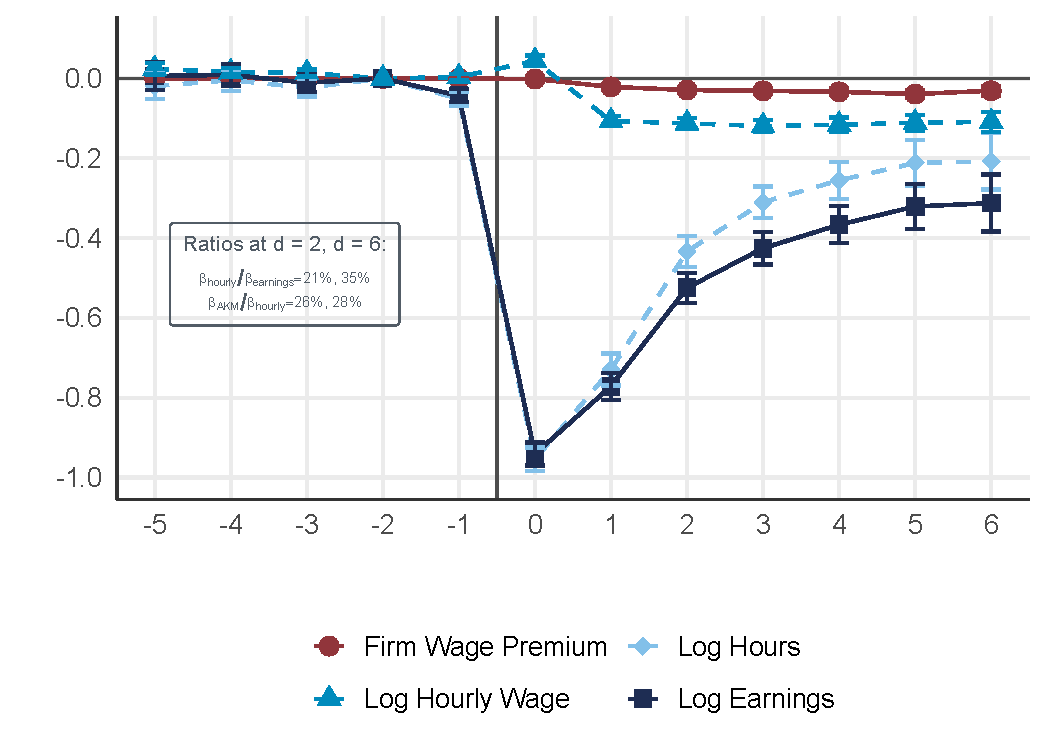
\includegraphics[width=0.75\linewidth, trim={0cm 0cm 0.1cm 0cm}, clip,max width=\linewidth]{figures/01_event_figures/figure_A8_a_men.pdf}
\end{subfigure}

\medskip

\begin{subfigure}[b]{\textwidth}
\centering
\caption*{\small (b) Women}
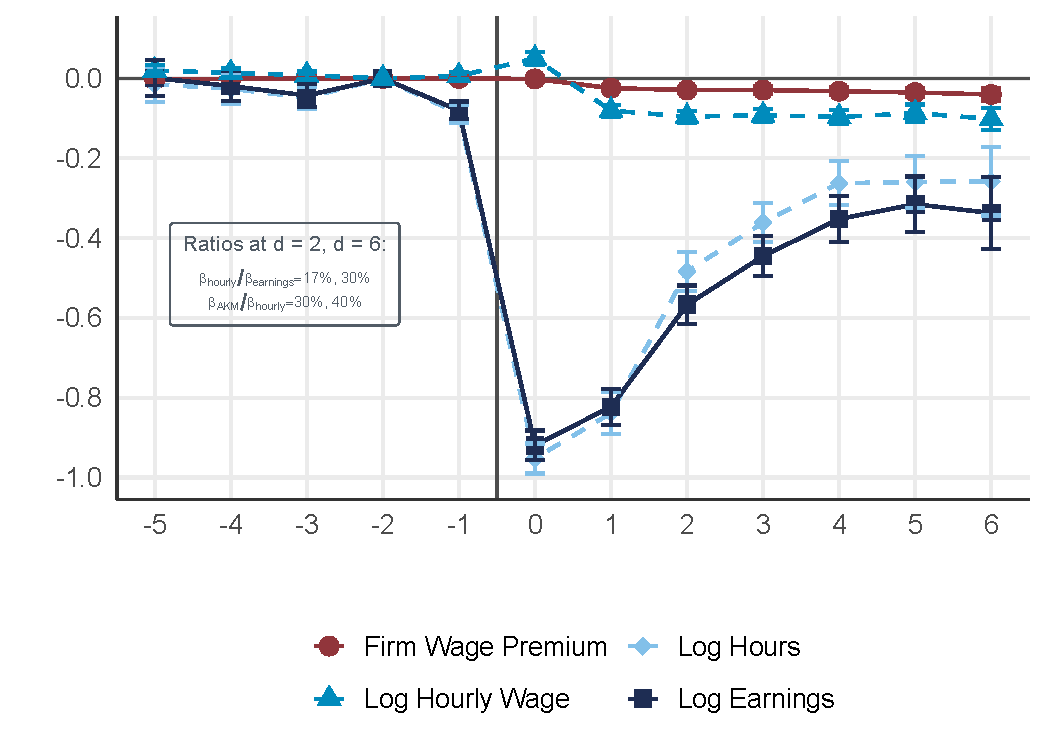
\includegraphics[width=0.75\linewidth, trim={0cm 0cm 0.1cm 0cm}, clip,max width=\linewidth]{figures/01_event_figures/figure_A8_b_women.pdf}
\end{subfigure}

\floatfoot{\footnotesize{\textsc{Notes}: This figure reproduces Figure~\ref{fig:fe_current_event} of the paper for men and women separately, on the LE sample. Men and women display similar profiles on the four outcomes: the hourly-wage scar at $t^D+5$ is $-0.105$ for men against $-0.089$ for women, and the AKM firm-premium scar is $-0.041$ for men against $-0.045$ for women. The hours and total-earnings scars are slightly larger for men than for women. \textbf{Sample}: $n_{\text{men}} = $ men, $n_{\text{women}} = $ women in the LE sample. \textbf{Standard errors}: robust standard errors clustered at the worker level; displayed confidence intervals at the $99\%$ level.}}
\end{figure}

\FloatBarrier

\begin{figure}[h!]
	\caption{Firms characteristics over the full period 2002--2015, LE sample \label{fig:prod_et_al_Full_LE}}
	\centering
	\begin{subfigure}[b]{.49\textwidth}
		\centering
		\caption[]{\small Productivity}
		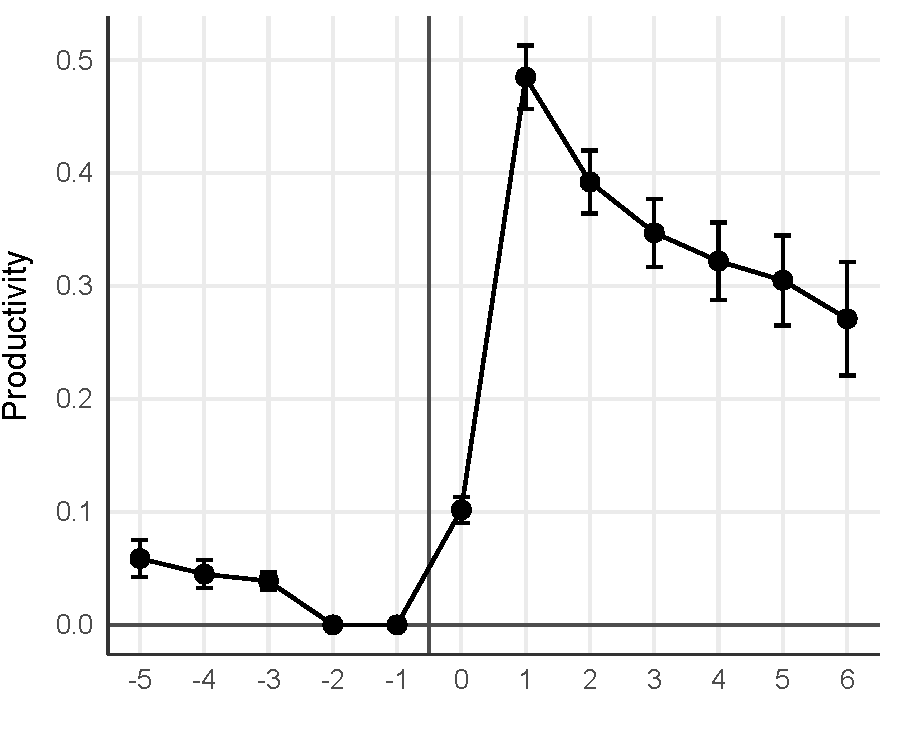
\includegraphics[scale=0.49,max width=\linewidth]{figures/01_event_figures/figure_A9_a_productivity.pdf}
	\end{subfigure}
	\begin{subfigure}[b]{.49\textwidth}
		\centering
		\caption[]{\small Log of value-added per worker}
		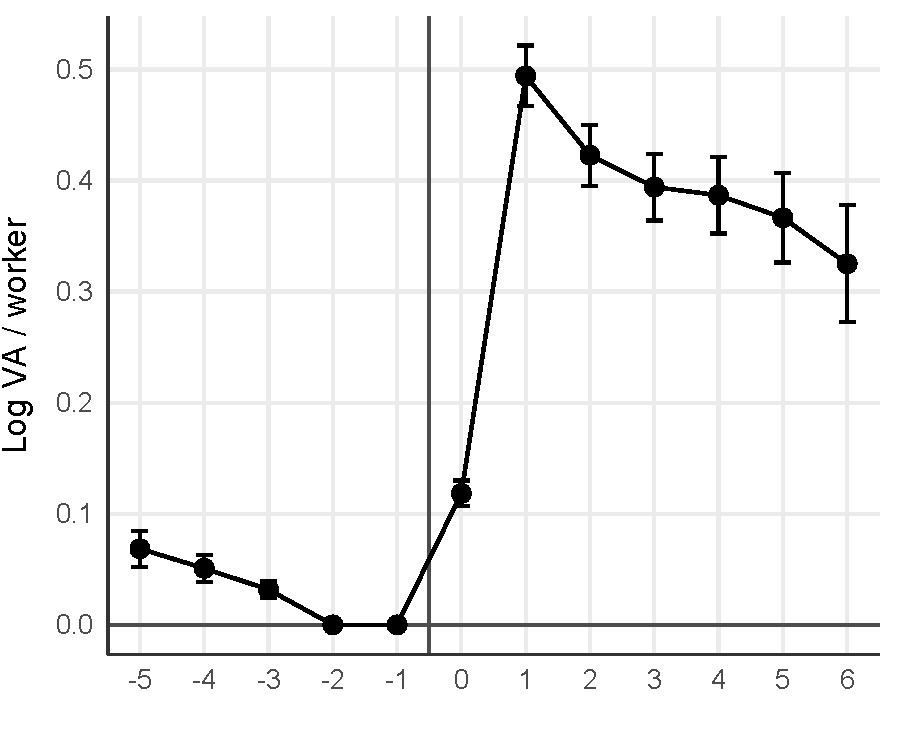
\includegraphics[scale=0.49,max width=\linewidth]{figures/01_event_figures/figure_A9_b_va_per_worker.pdf}
	\end{subfigure}
	\begin{subfigure}[b]{.49\textwidth}
		\centering
		\caption[]{\small Log of labor share of value-added}
		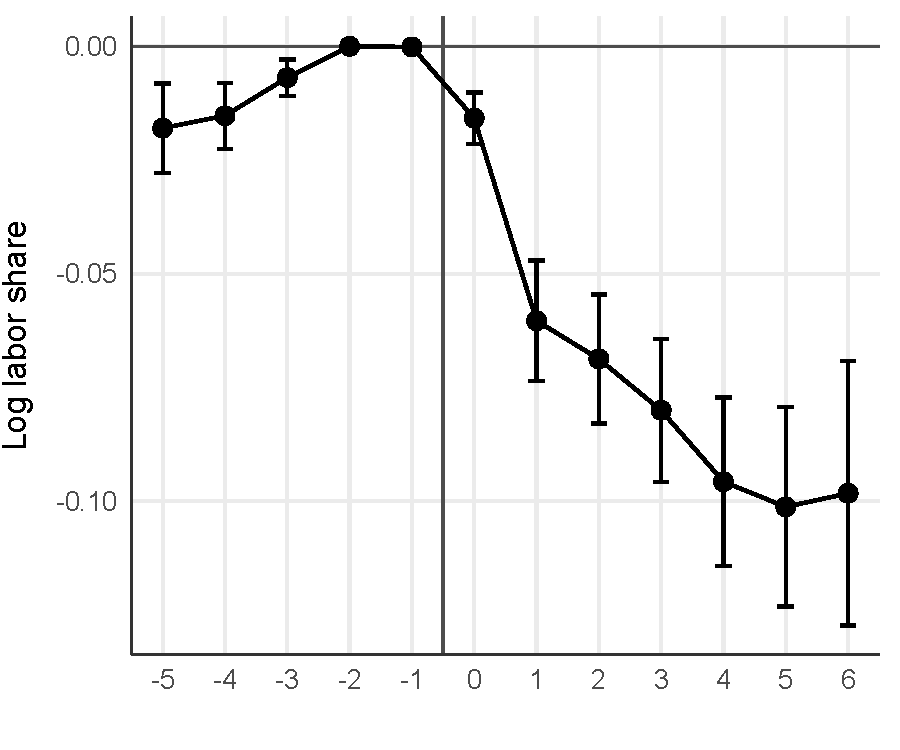
\includegraphics[scale=0.49,max width=\linewidth]{figures/01_event_figures/figure_A9_c_labor_share.pdf}
	\end{subfigure}
	\floatfoot{\footnotesize{\textsc{Notes}: This figure reports event-study estimates of the effect of job displacement on the reallocation of workers towards firms with varying levels of productivity, value added per workers and labor share. Coefficients are obtained by estimating the specification of equation \ref{eq:main_estimating_equation} where the dependent variable is sequentially productivity, value added per worker and labor share. \textbf{Sample}: The sample contains 8,341 individuals laid-off for economic reasons who end-up being re-employed post-displacement. Productivty can be estimated for only 7,524 of those. \textbf{Comment on timing}: Firm-level outcomes are computed as the average of the firm-level outcome over the full period 2002--2015, while displacements occurs at $t^D$ (with $t^D$ between 2005 and 2012). Accordingly, event-study coefficients reflect the movement of displaced workers to firms with different time-invariant characteristics and \textit{not} changes within-firm in such characteristics. \textbf{Definition of firm-level outcomes}: Table \ref{apptab:definitions} summarizes variables' definition. Value added per worker is computed as value added over reported employment. Productivity is obtained as the residual of an OLS regression of value-added on the book value of tangible capital and labor with year fixed effects. The labor share is computed as total labor cost over value-added, averaged over 2002--2015.  \textbf{Standard errors}: robust standard errors clustered at the worker-level; displayed confidence intervals at the 99\% level.}}
\end{figure}



\begin{figure*}[h!]
	\caption{Firms characteristics over the full period 2002--2015, MLO sample \label{fig:prod_et_al_Full_MLO}}
	\centering
	\begin{subfigure}[b]{.49\textwidth}
		\centering
		\caption[]{\small Productivity}
		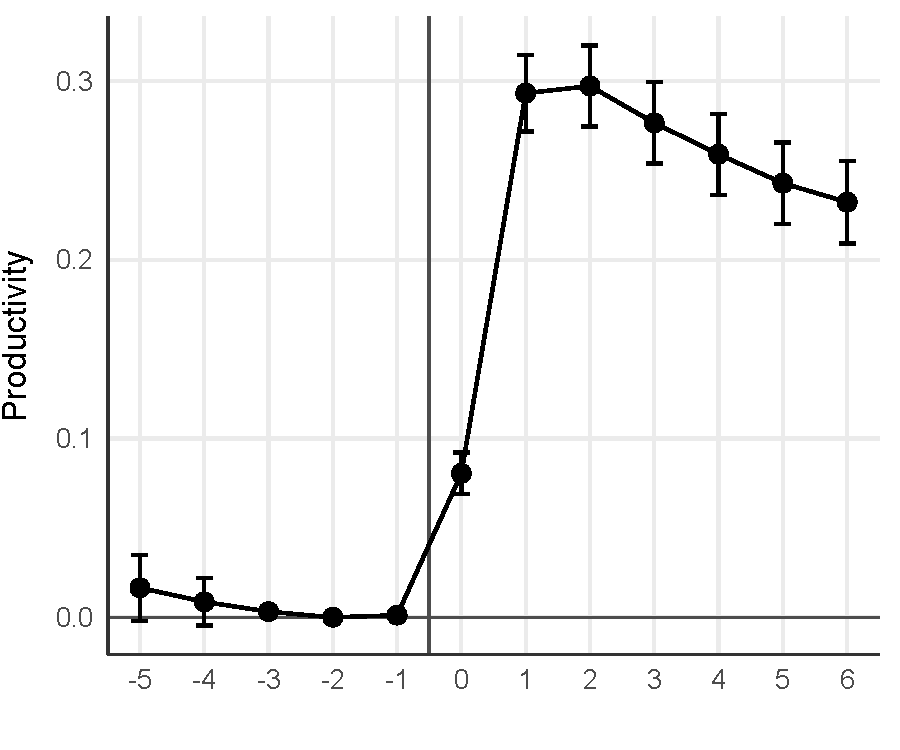
\includegraphics[scale=0.49,max width=\linewidth]{figures/01_event_figures/figure_A10_a_productivity.pdf}
	\end{subfigure}
	\begin{subfigure}[b]{.49\textwidth}
		\centering
		\caption[]{\small Log of value-added per worker}
		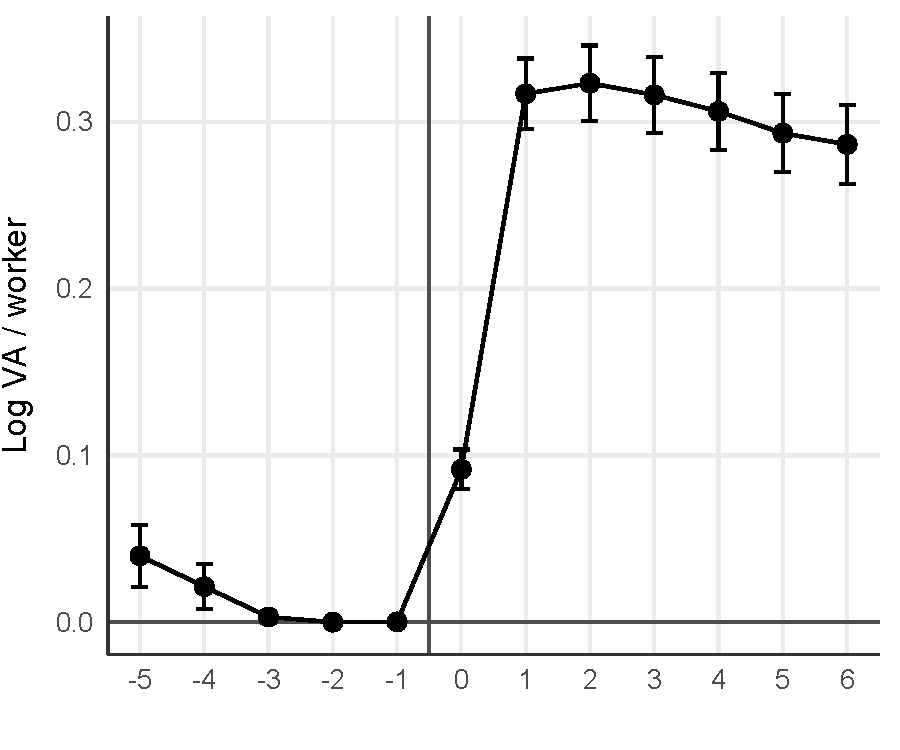
\includegraphics[scale=0.49,max width=\linewidth]{figures/01_event_figures/figure_A10_b_va_per_worker.pdf}
	\end{subfigure}
	\begin{subfigure}[b]{.49\textwidth}
		\centering
		\caption[]{\small Log of labor share of value-added}
		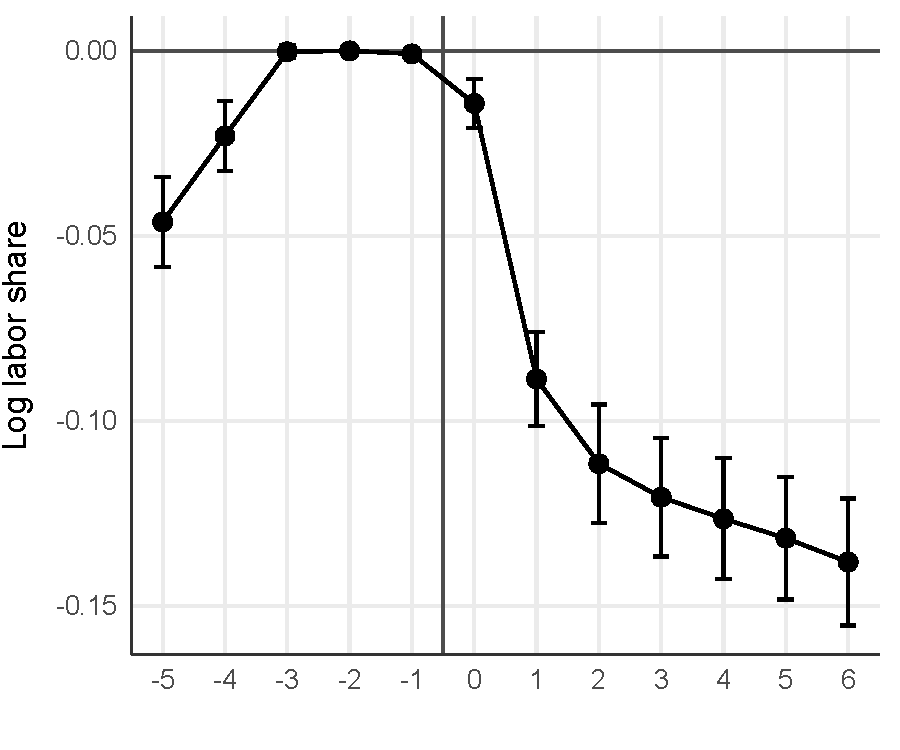
\includegraphics[scale=0.49,max width=\linewidth]{figures/01_event_figures/figure_A10_c_labor_share.pdf}
	\end{subfigure}
	\floatfoot{\footnotesize{\textsc{Notes}: This figure reports event-study estimates of the effect of job displacement on the reallocation of workers towards firms with varying levels of productivity, value added per workers and labor share. Coefficients are obtained by estimating the specification of equation \ref{eq:main_estimating_equation} where the dependent variable is sequentially productivity, value added per worker and labor share. \textbf{Sample}: The sample contains 4,772 individuals laid-off for economic reasons who end-up being re-employed post-displacement. Productivty can be estimated for only 4,130 of those. \textbf{Comment on timing}: Firm-level outcomes are computed as the average of the firm-level outcome over the full period 2002--2015, while displacements occurs at $t^D$ (with $t^D$ between 2005 and 2012). Accordingly, event-study coefficients reflect the movement of displaced workers to firms with different time-invariant characteristics and \textit{not} changes within-firm in such characteristics. \textbf{Definition of firm-level outcomes}: Table \ref{apptab:definitions} summarizes variables' definition. Value added per worker is computed as value added over reported employment. Productivity is obtained as the residual of an OLS regression of value-added on the book value of tangible capital and labor with year fixed effects. The labor share is computed as total labor cost over value-added, averaged over 2002--2015.  \textbf{Standard errors}: robust standard errors clustered at the worker-level; displayed confidence intervals at the 99\% level.}}
\end{figure*}



\begin{figure}[h!]
	\caption{Firm-level event-study of laying-off firms' productivity, LE sample \label{fig:firm_es_productivity}}
	\centering
	\begin{subfigure}[b]{.49\textwidth}
		\centering
		\caption[]{\small Residual productivity}
		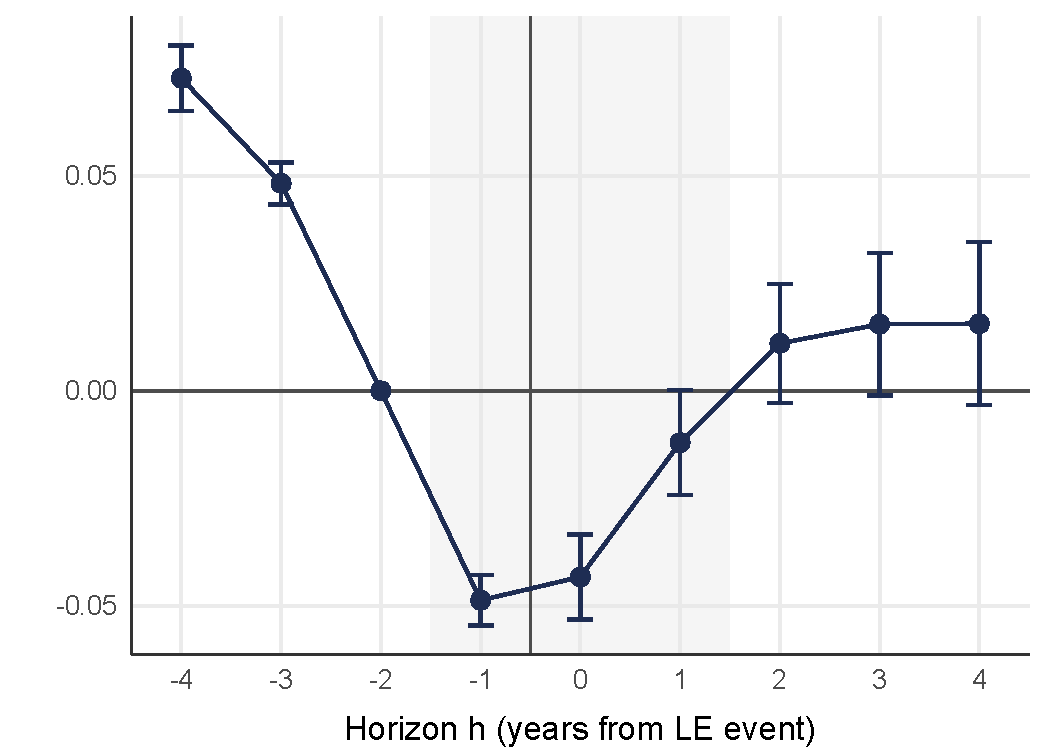
\includegraphics[scale=0.49,max width=\linewidth]{figures/01_event_figures/figure_A11_a_layoff_firm_productivity.pdf}
	\end{subfigure}
	\begin{subfigure}[b]{.49\textwidth}
		\centering
		\caption[]{\small TFP (Cobb--Douglas)}
		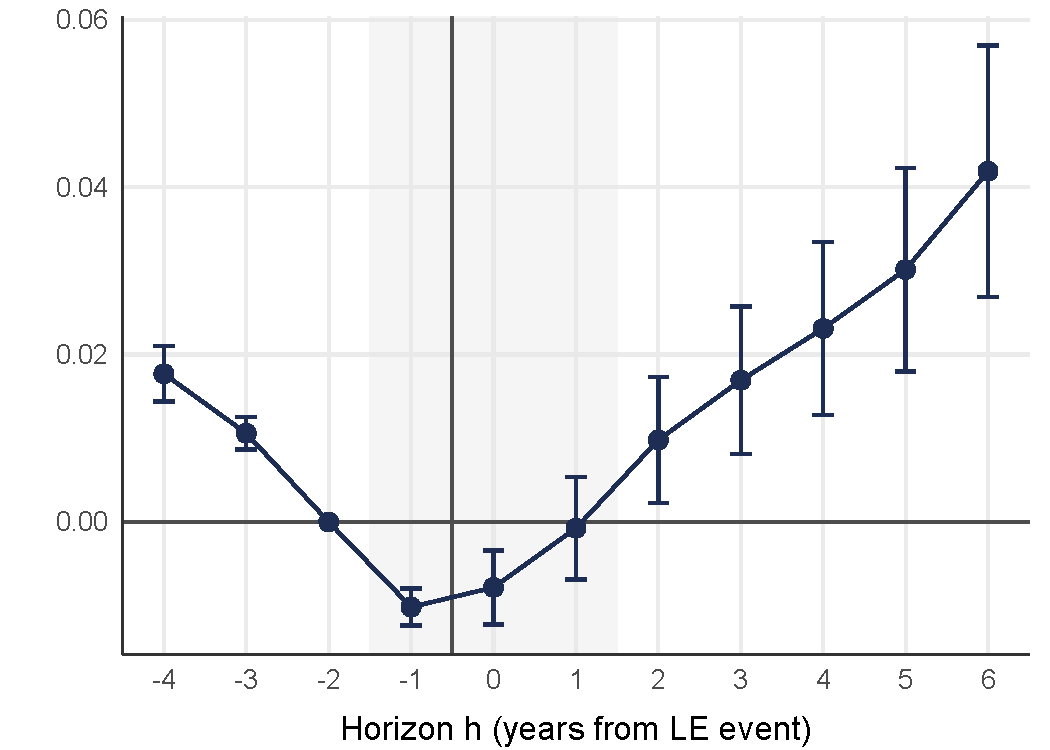
\includegraphics[scale=0.49,max width=\linewidth]{figures/01_event_figures/figure_A11_b_layoff_firm_tfp.pdf}
	\end{subfigure}
	% \begin{subfigure}[b]{.49\textwidth}
	% 	\centering
	% 	\caption[]{\small TFP (translog)}
	% 	\includegraphics[scale=0.49,max width=\linewidth]{figures-2026/firm_es_tfp_tl.pdf}
	% \end{subfigure}
	\floatfoot{\footnotesize{\textsc{Notes}: This figure reports event-study estimates from a firm-level event study where the unit of observation is the firm (\textit{not the worker}). Treated firms ($n=8{,}001$) are firms experiencing their first economic-layoff event between 2005 and 2012 (LE sample); the omitted reference horizon is $h=-2$. The dependent variables are 3-year moving averages of firm-level productivity centered on year $t$, i.e.\ averaged over $[t-1, t, t+1]$. Horizons $h \in \{-1, 0, +1\}$ (shaded) overlap with the layoff year and should be interpreted as a transition window; horizons $h \geq +2$ are the first windows containing only post-layoff years. Panel (a) plots the results for the residual of an OLS regression of value-added on tangible capital and labor with year fixed effects; panel (b) plots the results for Cobb--Douglas TFP estimates, imposing common factor coefficients across firms within 2-digit sectors. Standard errors are clustered at the firm level; displayed confidence intervals are at the 99\% level.}}
\end{figure}



\begin{figure}[h!] \centering
	\caption{Firm-specific wage premium and productivity \label{fig:bscatter_firmfe_prod}}
	\begin{subfigure}[b]{.49\textwidth}
		\centering
		\caption[]{\small Value-added per worker} \label{fig:firm_LE_binscatter_ln_apl}
		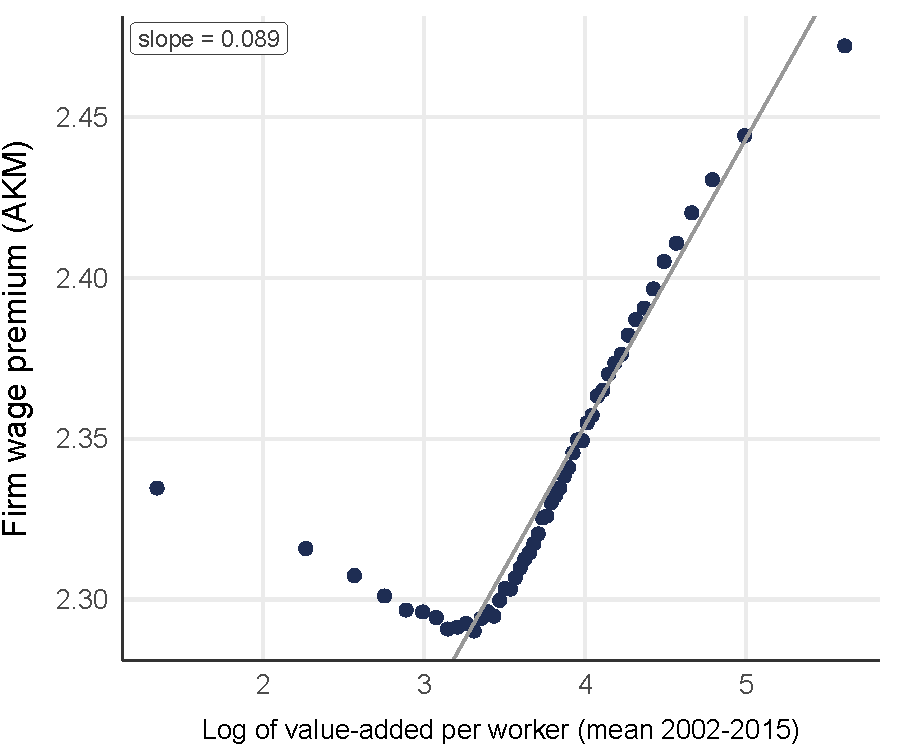
\includegraphics[scale=0.49,max width=\linewidth]{figures/02_descriptive_figures/figure_A12_a_va_per_worker.pdf}
	\end{subfigure}
	\begin{subfigure}[b]{.49\textwidth}
		\centering
		\caption[]{\small Productivity} \label{fig:firm_LE_binscatter_prod_res}
		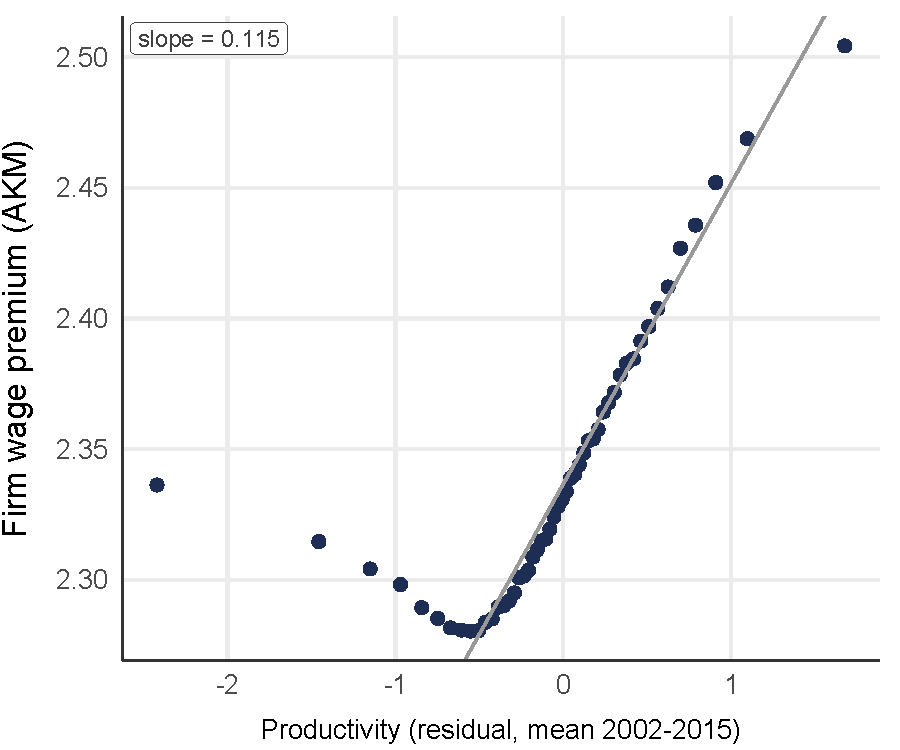
\includegraphics[scale=0.49,max width=\linewidth]{figures/02_descriptive_figures/figure_A12_b_productivity.pdf}
	\end{subfigure}
	
	\floatfoot{\footnotesize{\textsc{Notes}: This figure displays the binned scatter plot of firm-premia with respect to (log) value-added per worker (left panel) and productivity (right panel). 50 quantiles are used. The linear fit (light gray line) is estimated on a sample excluding the bottom 5 and the top 1 quantiles. As in the Portuguese data \citep[][see in particular Figure IV, page 663]{card2016bargaining}, the firm AKM fixed-effects and value-added per worker (or productivity) are strongly positively associated outside of the bottom of the distribution.  Fitted slope=0.085 (left) and 0.095 (right). \textcolor{orange}{[0.089 and 0.115, as printed on the R2 figure]} \textbf{Definition of variables}: Table \ref{apptab:definitions} summarizes variables' definition. Value-added per worker is computed as value-added over reported employment. Productivity is obtained as the residual of an OLS regression of value-added on the book value of tangible capital and labor with year fixed effects, where value-added is deflated using 2-digit value added deflator (\textit{Indice de prix de la valeur ajoutée brute par branche}). }} 
\end{figure}


\begin{figure}[h!] \centering
	\caption{Firm-specific wage premium and bargaining outcomes\label{fig:bscatter_firmfe_bargaining}}
	\begin{subfigure}[b]{.49\textwidth}
		\centering
		\caption[]{\small Indicator of wage agreement} \label{fig:firm_LE_binscatter_wage_agreement}
		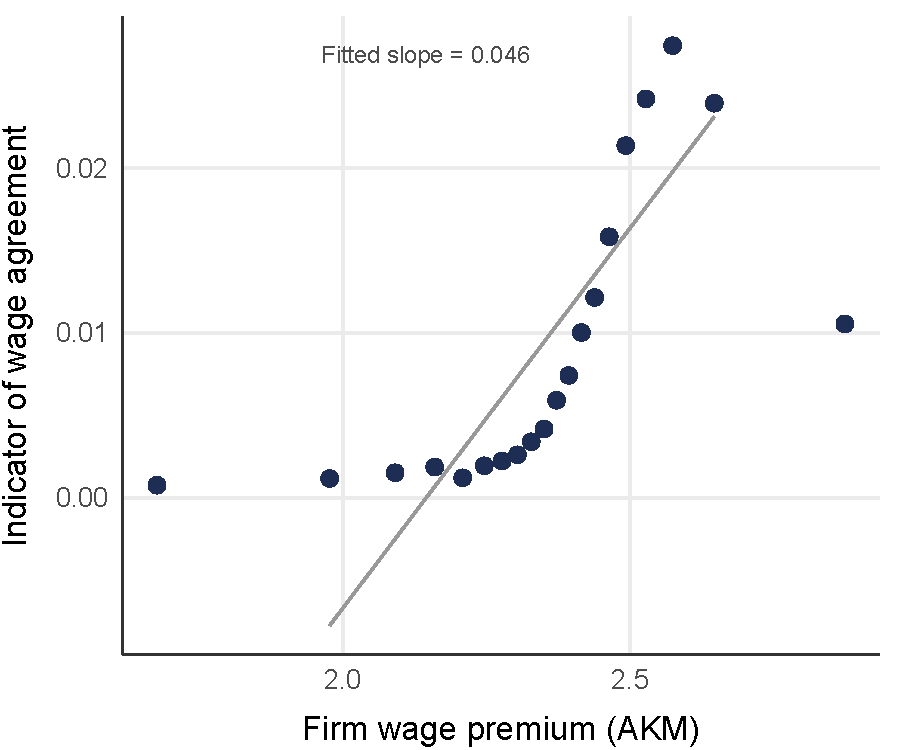
\includegraphics[scale=0.49,max width=\linewidth]{figures/02_descriptive_figures/figure_A13_a_wage_agreement.pdf}
	\end{subfigure}
	\begin{subfigure}[b]{.49\textwidth}
		\centering
		\caption[]{\small Election turnout} \label{fig:firm_LE_binscatter_election_turnout}
		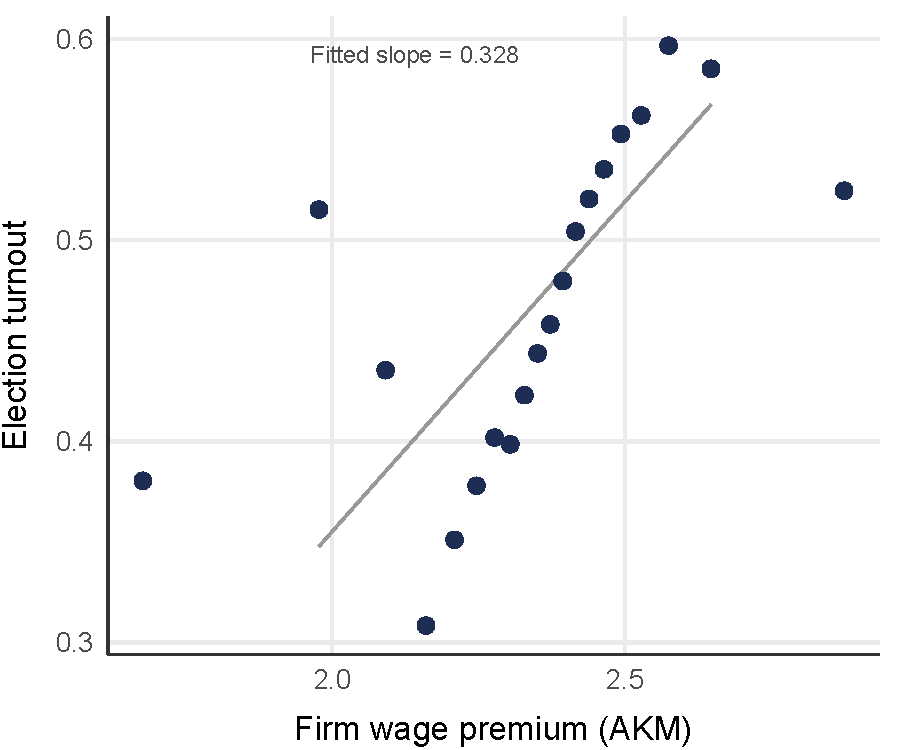
\includegraphics[scale=0.49,max width=\linewidth]{figures/02_descriptive_figures/figure_A13_b_election_turnout.pdf}
	\end{subfigure}

	\floatfoot{\footnotesize{\textsc{Notes}: This figure complements Figure~\ref{fig:bscatter_firmfe_prod} by showing the binned scatter plot of two firm-level bargaining outcomes against the firm-specific AKM premium $\widehat\psi_f$ (contamination-corrected): an indicator of wage-agreement signing over 2005--2007 (panel a) and the firm-level average turnout at 2009--2012 workplace elections (panel b). Firms are grouped into 20 quantiles of $\widehat\psi_f$. Linear fits (light gray) are estimated excluding the bottom and top quantile bins. Both bargaining outcomes are strongly positively associated with the firm wage premium (fitted slopes: $0.586$ for wage agreement, $0.298$ for election turnout) \textcolor{orange}{[0.046 and 0.328, as printed on the R2 figure; with 0.046 the agreement indicator is no longer ``strongly'' associated with the premium---reword]}, suggesting that worker bargaining power is one of the firm-level dimensions captured by the AKM premium. \textbf{Definition of variables}: see Table~\ref{apptab:definitions} for full definitions; the wage-agreement indicator equals one if the firm signed at least one wage-related agreement over 2005--2007, and election turnout is the firm-level average turnout at 2009--2012 workplace elections.}}
\end{figure}

\begin{figure}[h!] \centering
	\caption{Distribution of firm fixed effects in the sample of displaced workers: comparison with previous work \label{fig:sample_FEdist}}
		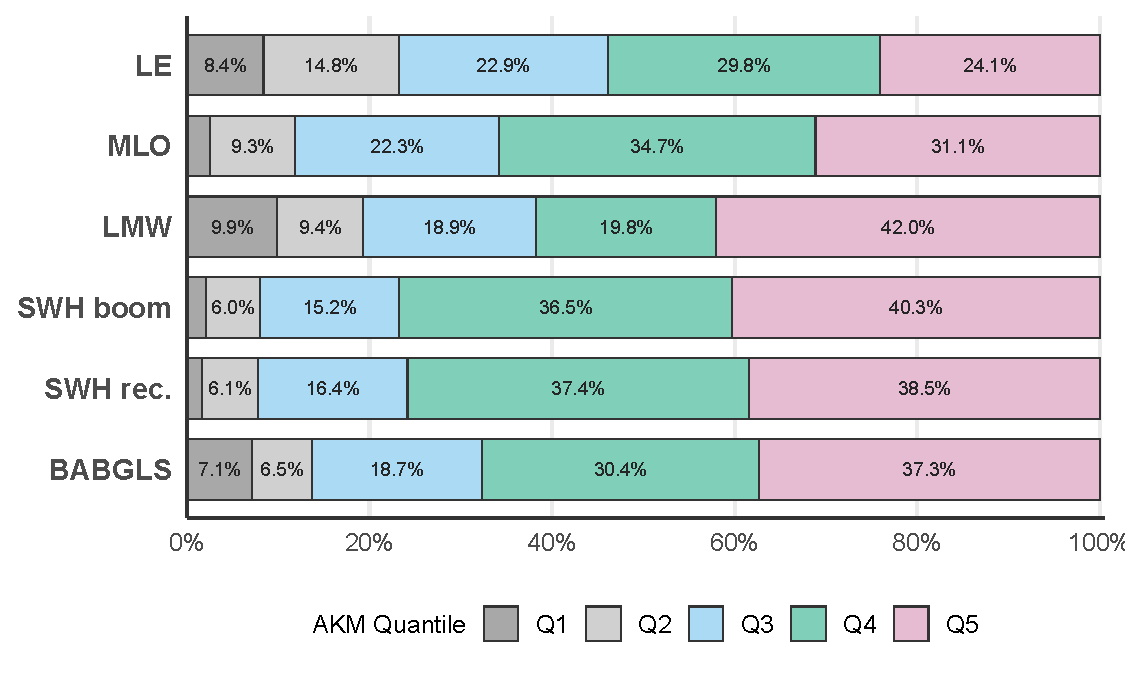
\includegraphics[width=\linewidth,max width=\linewidth]{figures/02_descriptive_figures/figure_A14_firm_premium_distribution.pdf}
	
	\floatfoot{\footnotesize{\textsc{Notes}: This figure displays the distribution of the firm AKM fixed-effects in the estimating sample. It presents the share of observations falling into each of the five quintiles of the AKM distribution (computed on the population of firms) for our economic-layoff sample (LE) and our mass-layoff sample (MLO30). For comparison we also report the corresponding figures from related papers in the displacement literature: LMW \citep{Lachowska2020}; SWH \citep{Schmieder2020}, for which we distinguish boom and recession episodes; and BABGLS \citep{bertheau_etal_2023}. In the first row (LE), 55.9\% of displaced workers come from firms in the top two quintiles \textcolor{orange}{[53.9\%, as printed on the R2 figure]} of the AKM premium distribution---above the 40\% benchmark a fully representative sample would deliver, indicating moderate over-representation of high-premium firms. The MLO row is more skewed: the corresponding share is 67.7\% \textcolor{orange}{[65.8\%]}, consistent with the fact that mass-layoff events tend to occur disproportionately in larger and higher-premium firms. The four remaining rows put these numbers in perspective: in all comparable papers, the share of displaced workers in the top two quintiles is at least as high as in our MLO sample (61.8\% in LMW, 75.9--76.8\% in SWH boom and recession, 67.7\% in BABGLS), and our LE sample is the least skewed of all six. The over-representation of high-premium firms is therefore noticeably milder in our LE design than in the rest of the literature.}}
\end{figure}



\begin{figure}[h!] 
	\caption{Raw Means on Earnings in Control and Treatment Groups\label{fig:raw_mean_earnings}} 
	\centering
	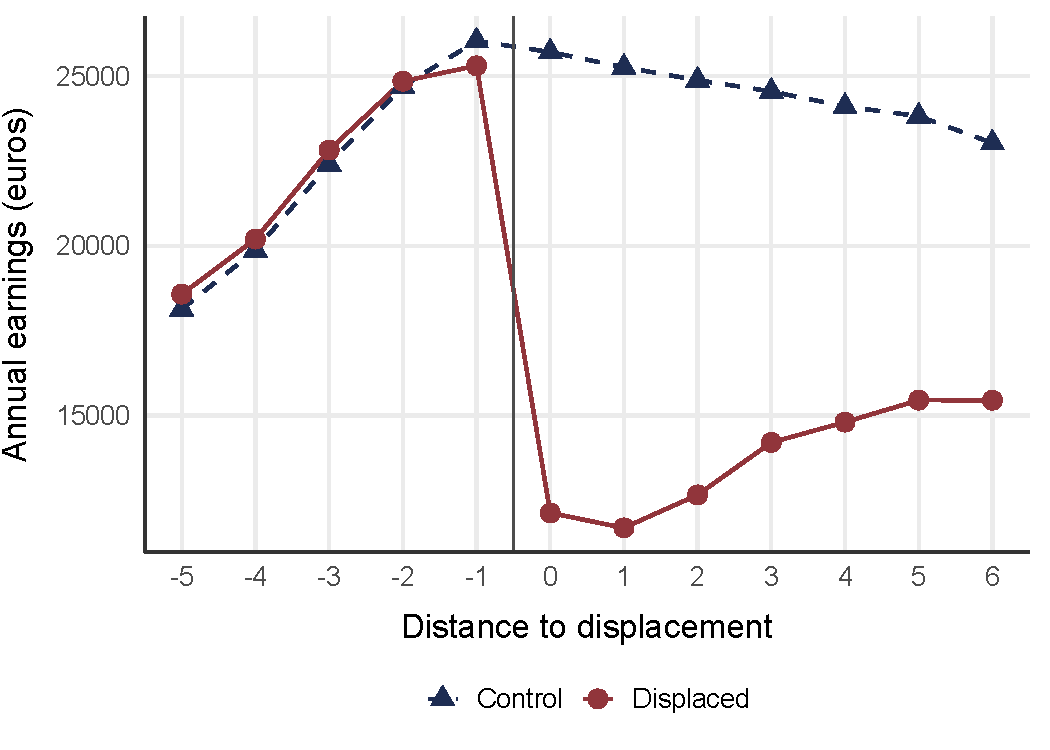
\includegraphics[scale=0.75,max width=\linewidth]{figures/02_descriptive_figures/figure_A15_raw_earnings.pdf}
\floatfoot{\footnotesize{\textsc{Notes}: This figure displays the average annual gross wage in both displaced-workers and control groups. It shows the evolution of gross wage in our sample from $t^D-3$ to $t^D+6$. \textbf{Sample}: The sample contains 20,897 economic dismissals (LE) and as many controls. \textcolor{orange}{[21,132]} \textbf{Outcomes:} Table \ref{apptab:definitions} summarizes variables' definition. \textbf{Specification}: The points displayed are computed as the simple average in annual gross wage by distance to displacement. Non working individuals have wage 0 (as long as they are under 65 and $t<2013$).
}}
\end{figure}


\begin{figure}[h!] 
	\caption{Raw Means on Hours Workers in Control and Treatment Groups\label{fig:raw_mean_hours}} 
	\centering
	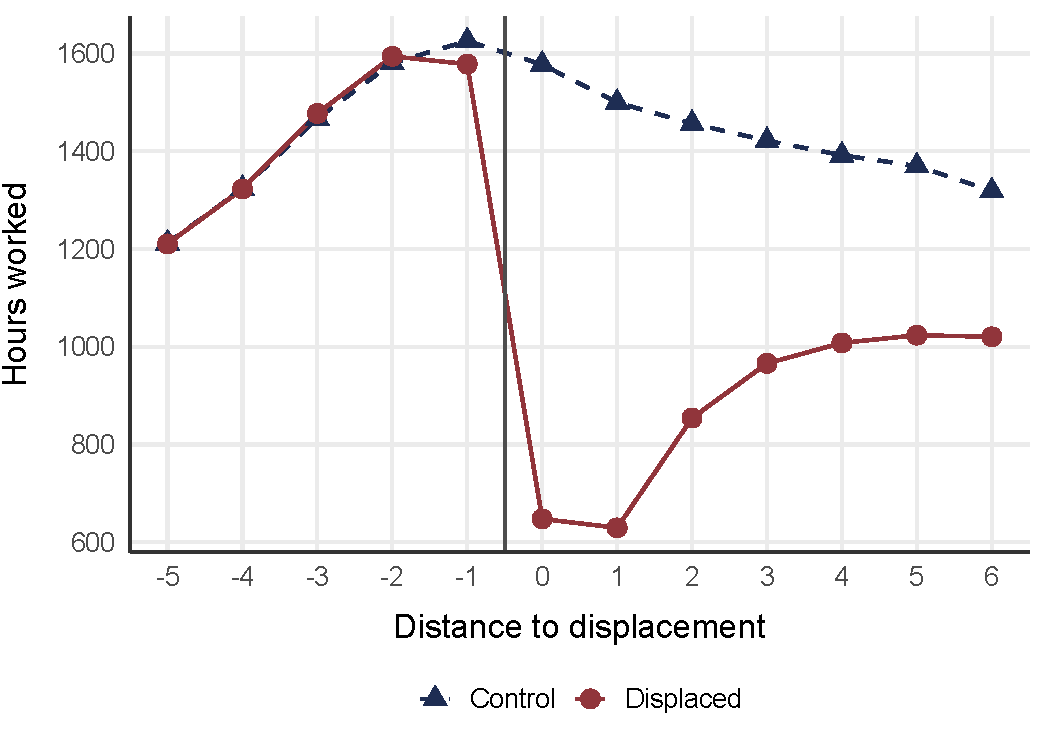
\includegraphics[scale=0.75,max width=\linewidth]{figures/02_descriptive_figures/figure_A16_raw_hours.pdf}
\floatfoot{\footnotesize{\textsc{Notes}: This figure displays the average number of hours worked in both displaced-workers and control groups. It shows the evolution of hours in our sample from $t^D-3$ to $t^D+6$. \textbf{Sample}: The sample contains 20,897 economic dismissals (LE) and as many controls. \textcolor{orange}{[21,132]} \textbf{Outcomes:} Table \ref{apptab:definitions} summarizes variables' definition. \textbf{Specification}: The points displayed are computed as the simple average in annual hours worked by distance to displacement. Non working individuals have hours 0 (as long as they are under 65 and $t<2013$).
}}
\end{figure}




\FloatBarrier
\clearpage

\subsection{Tables}
\FloatBarrier

\begin{table}[h!]
\centering
\caption{Raw firm-level means by type of firm (LE sample, descriptive complement to Table~\ref{tab:firing_hiring_rest})\label{apptab:firing_hiring_means}}
{\footnotesize
\begin{adjustbox}{max width=\linewidth}
\begin{tabular}{lcccccc}\toprule
% Generated from current results_analysis CSV files by master.R, section I (scripts/I-PLOTS_AND_TABLES).
% Table A1; status: ready
% Cell means weighted by n_siren; overlapping firms appear in both rows. Outcome-specific nonmissing denominators are not exported.
% -- means a requested statistic is unavailable; an empty cell means not applicable.
 & (1) & (2) & (3) & (4) & (5) & (6) \\
 & Wage premium & ln(VA/L) & Productivity & ln(labor share) & ln(L) & N (firms) \\
\midrule
Origin firms & 2.429 & 3.704 & -0.037 & -0.127 & 2.688 & 14,115 \\
Destination firms & 2.433 & 4.011 & 0.172 & -0.223 & 3.237 & 5,076 \\
Other firms & 2.340 & 3.743 & -0.070 & -0.318 & 0.976 & 1,897,770 \\

\bottomrule
\end{tabular}
\end{adjustbox}}
\floatfoot{\footnotesize{\textsc{Notes}: Raw firm-level means for three exhaustive groups of firms in the FICUS-FARE panel: (i) origin firms (where displaced workers were employed in $t^D-1$), (ii) destination firms (where displaced workers were employed in $t^D+4$ or $t^D+5$), and (iii) the population of firms that are neither an origin nor a destination of any LE-displaced worker. The Origin and Destination groups overlap in $497$ firms (about $3.5\%$ of origins and $9.7\%$ of destinations) \textcolor{orange}{[R2: 490 firms, since $14{,}115+5{,}076+1{,}897{,}770-1{,}916{,}471=490$ (group sizes in this table, observations in Table~\ref{tab:firing_hiring_rest}); the same identity gives the 497 of R1; the two shares still round to 3.5\% and 9.7\%]}; these firms are counted in both rows. All firm-level outcomes are computed as the within-firm average over $2002$--$2015$. ``Wage premium'' is $\widehat{\psi}_{f}$ from Section~\ref{sec:data:firm:premium}, estimated on the entire panel; productivity is the residual from an OLS regression of value-added on tangible capital and labor with year fixed effects. \textcolor{orange}{The raw means already show that destination firms are more productive than origin firms ($+0.172$ against $-0.037$), and that both groups pay higher wage premia than other firms ($2.433$ and $2.429$ against $2.340$); the premium gap between origin and destination firms highlighted in Table~\ref{tab:firing_hiring_rest} appears once sectors are controlled for.}}}
\end{table}

\FloatBarrier

\begin{table}[h!]
\centering
\caption{Comparison of origin and destination firms, weighted by firm employment (worker-level analogue of Table~\ref{tab:firing_hiring_rest})\label{apptab:firing_hiring_weighted}}
{\footnotesize
\begin{adjustbox}{max width=\linewidth}
\begin{tabular}{llll}\toprule
% Generated from current results_analysis CSV files by master.R, section I (scripts/I-PLOTS_AND_TABLES).
% Table A2; status: ready
% Adjusted R2 and the origin-destination equality-test p-value use the updated exports.
% -- means a requested statistic is unavailable; an empty cell means not applicable.
 & (1) & (2) & (3) \\
 & Wage premium & VA/worker & Productivity \\
\midrule
Destination firm & 0.01958\sym{***} & 0.07059\sym{***} & 0.05514\sym{**} \\
 & (4.11) & (3.39) & (3.00) \\
\addlinespace
Origin firm & 0.04297\sym{***} & 0.01066 & 0.01285 \\
 & (5.39) & (0.97) & (1.46) \\
\addlinespace
\midrule
Observations & 1,916,471 & 1,916,471 & 1,916,471 \\
$R^2$ & 0.173 & 0.338 & 0.269 \\
Adjusted $R^2$ & 0.173 & 0.338 & 0.269 \\
Sector FE & $\surd$ & $\surd$ & $\surd$ \\
P-value Origin-Destination & 0.053 & 0.041 & 0.089 \\

\bottomrule
\end{tabular}
\end{adjustbox}}
\floatfoot{\footnotesize{\textsc{Notes}: This table reproduces the structure of Table~\ref{tab:firing_hiring_rest} columns (1) to (3) for the same outcomes (firm wage premium, value-added per worker, productivity), but the regressions are weighted by firm employment ($\exp(\overline{\ln L_{f}})$ averaged over 2001--2015). Because in a firm-level cross-section the weighted firm-mean coincides with the unweighted worker-level mean, the table is equivalent to running the comparison at the worker level relative to an average worker, as suggested by a referee. The qualitative pattern is preserved relative to Table~\ref{tab:firing_hiring_rest}: origin firms have higher wage premia and lower value added per worker than destination firms. \textcolor{orange}{[``similar magnitudes'' clause dropped on 2026-11-20: the premium gap between origin and destination firms is larger when firms are weighted, as Section~\ref{sec:rolefirm:hiring_firing} now states]} $z$-statistics based on robust standard errors in parentheses. {*} $p<0.05$, {**} $p<0.01$, {***} $p<0.001$.}}
\end{table}

\FloatBarrier

% Added in the R2 revision (Referee 3, point 4): dispersion of firm-level characteristics across firms.
% The tabular is shared with Table R2 of the letter to Referee 3 (Letters/referee3_response.tex).
\begin{table}[h!]\caption{Dispersion of firm-level characteristics across firms, 2002--2015 averages}\label{apptab:dispersion}
	{\footnotesize
	\begin{center}
		\begin{adjustbox}{max width=\linewidth}
		% Generated from current results_analysis CSV files by master.R, section I (scripts/I-PLOTS_AND_TABLES).
% Table A3; status: ready
% Employment-weighted moments; baseline LE effects at +5; percentile approximated from adjacent quartiles.
% -- means a requested statistic is unavailable; an empty cell means not applicable.
\begin{tabular}{lcccc}
\toprule
 & (1) & (2) & (3) & (4) \\
 & Productivity & VA per worker & Labor share & Wage premium \\
\midrule
\multicolumn{5}{l}{\textit{Panel A. Distribution across firms, weighted by employment}} \\
Standard deviation & 0.601 & 0.688 & 0.481 & 0.173 \\
25th percentile & -0.171 & -0.199 & -0.015 & 0.029 \\
Median & 0.090 & 0.097 & 0.194 & 0.119 \\
75th percentile & 0.436 & 0.452 & 0.336 & 0.198 \\
Interquartile range & 0.607 & 0.652 & 0.352 & 0.168 \\
\addlinespace
\multicolumn{5}{l}{\textit{Panel B. Displacement effect at $t^D+5$ (Table~\ref{tab:evstudytable_body}) relative to panel A}} \\
Coefficient at $t^D+5$ & 0.134 & 0.066 & -0.074 & -0.037 \\
Share of the interquartile range & 0.22 & 0.10 & 0.21 & 0.22 \\
In standard-deviation units & 0.22 & 0.10 & 0.15 & 0.22 \\
Percentile reached by a median firm & 60 & 55 & 41 & 40 \\
\midrule
Firms with a non-missing value & 2,346,321 & 2,525,260 & 2,534,596 & 2,054,893 \\
\bottomrule
\end{tabular}

		\end{adjustbox}
	\end{center}}
	\floatfoot{{\footnotesize \textsc{Notes}: Each column reports the distribution across firms of one firm-level characteristic, computed as a within-firm average over 2002--2015. \textcolor{orange}{Each column uses all firms of the FICUS-FARE data with non-missing employment and a non-missing value of that characteristic (last row). Table~\ref{tab:firing_hiring_rest} instead keeps only firms with non-missing values for all its outcomes, hence its smaller sample.} \textit{Productivity} is the residual of an OLS regression of log value added on log tangible capital and log employment with year fixed effects, net of 2-digit sector fixed effects -> \textcolor{red}{without additional 2-digit sector residualization}; \textit{VA per worker} is log value added per worker; \textit{labor share} is the log of total labor costs over value added; \textit{wage premium} is the AKM firm fixed effect estimated over 2002--2015 (Section \ref{sec:data:firm:premium}). All variables are expressed as deviations from their unweighted mean across firms. In panel A firms are weighted by employment. Panel B reports the $t^D+5$ coefficients of Table \ref{tab:evstudytable_body} (panel b for columns 1--3, column (6) of panel a for the wage premium), their absolute value as a share of the employment-weighted interquartile range and in employment-weighted standard-deviation units, and the percentile that a firm initially at the median of panel A would reach after a change equal to the coefficient, obtained by linear interpolation between the median and the adjacent quartile. The event-study outcomes are three-year averages centered on $t^D-4$, which are more dispersed across firms than the fourteen-year averages used here.}}
\end{table}

\FloatBarrier

\begin{table}[h!]
\centering
\caption{Event-study coefficients for firm age and worker mean tenure (LE sample) \label{apptab:firm_age_tenure}}
% Generated from current results_analysis CSV files by master.R, section I (scripts/I-PLOTS_AND_TABLES).
% Table A4; status: ready
% Tenure is mean_tenure_eqtp_ma3_dlag4 under the confirmed baseline rule.
% -- means a requested statistic is unavailable; an empty cell means not applicable.
\begin{tabular}{lcccc}
\toprule
 & $d=-2$ & $d=0$ & $d=2$ & $d=5$ \\
\midrule
Firm age (years) & +0.000 & -0.609*** & -2.124*** & -1.931*** \\
 &  & (0.076) & (0.218) & (0.337) \\
Mean worker tenure (years) & +0.000 & -0.110*** & -0.685*** & -0.444*** \\
 &  & (0.009) & (0.033) & (0.044) \\
\bottomrule
\end{tabular}

\floatfoot{\footnotesize{\textsc{Notes}: Event-study coefficients of the displacement indicator on two firm-level outcomes for the LE sample: the destination firm's age in years (defined as the year minus year of creation) and the firm-level mean of worker tenure in years. $d=-2$ is the reference period (coefficient implicitly zero). Standard errors clustered at the worker level in parentheses; significance: $^{*}p<0.10$, $^{**}p<0.05$, $^{***}p<0.01$. The destination--origin gap of $\approx -1.5$ years on firm age and $\approx +0.55$ years on mean tenure at $t^D+5$ is too small to substitute for the bargaining-power channel discussed in the paper.}}
\end{table}

\FloatBarrier

% The descriptive statistics table (former Table A4, label tab:desc:AllLE) was moved to the main text in the R2 revision (Referee 3, point 1).

\begin{table}
	\caption{Definition of datasets}\label{apptab:datasets}
	{\scriptsize% Generated from the current results_analysis CSV files by plots_tables/run_all.R.
% Table A5; status: ready
% Text definitions retained; no numerical regression results copied.
% -- means a requested statistic is unavailable; an empty cell means not applicable.
{
\begin{tabularx}{\textwidth}{ZXlZ}
\hline
Dataset & Description & Period & Main use \\
\hline
&&&\\
DADS postes & (\textit{Déclaration Annuelle des Données Sociales}) is a matched employer-employee dataset coming from the administrative declaration that all employers report annually to social security authorities and tax administration; we restrict the sample to companies governed by private law. DADS contains information on firms and establishments (unique identifier; size; industry) as well as on each employees’ job (occupation, wage, hours worked, start and end date, type of contract, etc.). Firm (SIREN) unique id. & ]2001-2015[ & Compute firm premium \\
\rowcolor{lightgray} Panel DADS & Is a panel version of DADS (cf. above) containing a random sample of 1/12 of the universe of workers. Firm (SIREN) and worker unique id. & ]2001-2015[ & Workers' trajectories. Samples construction. \\
FH-DADS  & Matches the Panel DADS (cf. above) to the FH (Fichier Historique) data, an historical administrative file produced by the national unemployment agency (\textit{Pôle Emploi}) which records individuals’ unemployment spells. Any job seeker claiming unemployment benefits appears in the FH, which contains information about date of registration, duration and level of unemployment benefits. Firm (SIREN) and worker unique id. & [2002-2012] & Identify workers laid-off for economic reasons \\
\rowcolor{lightgray} FICUS-FARE  & Is a nearly exhaustive administrative dataset built from the corporate tax returns and the social security declaration of the universe of firms in the non-financial corporate sector. We use the FICUS-FARE panel as processed by \citet{burstein_etal_2025}. Firm (SIREN) unique id. & ]2001-2015[ & Firms' productivity, value-added, etc. \\
D@ccord  & D@ccord data reports information about firms' negotiations regarding collective agreement. In France, firms are required by the labor law to report any negotiation (successfull or not). The Ministry of Labor then builds this data set. Useful information contains: the matter of negotiation (wages, hours, etc.), the parties negotiating or signing (trade union, etc.), outcome, date of signature. Firm (SIREN) unique id. & [2005-2007[ & Collective agreements. \\
\rowcolor{lightgray} Workplace election  & Data reports the results of all workplace election held in France over 2009-2012. The election is characterized by its electoral college and its outcome (share of voters, vote by trade union, etc.) Firm (SIREN) unique id. & [2009-2012] & Workplace election turnout and failure. \\
&&&\\ \hline
\end{tabularx}
}







}
	\floatfoot{{\footnotesize \textsc{Notes}: This table provides a summary of the main datasets.}}
\end{table}



\begin{table}
	\caption{Definition of main variables (1/2)}\label{apptab:definitions}
	{\footnotesize% Generated from the current results_analysis CSV files by plots_tables/run_all.R.
% Table A6; status: ready
% Text definitions retained; no numerical regression results copied.
% -- means a requested statistic is unavailable; an empty cell means not applicable.
{
%\def\sym#1{\ifmmode^{#1}\else\(^{#1}\)\fi}
\begin{tabularx}{\textwidth}{ZXlZ}
	%\begin{tabular}{l*{3}{c}}
\hline
%\multicolumn{1}{c}{Outcome}&\multicolumn{1}{c}{Definition}&\multicolumn{1}{c}{Period}&\multicolumn{1}{c}{Source}\\
Outcome & Definition & Period & Source\\
\hline
&&&\\
\multicolumn{4}{l}{\textbf{Worker}} \\ 
Employed  & Indicator taking value 1 if the workers has worked (positive hours and earning). & $t$ & DADS panel \\
\rowcolor{lightgray} Earnings & Total of gross wages earned by the worker. Missing data is coded 0. & $t$ & DADS panel \\
Hours worked  & Total hours worked by the worker. Missing data is coded 0.  & $t$ & DADS panel \\
\rowcolor{lightgray} Hourly wage (or wage rate)  & Earnings over Hours. & $t$ & DADS panel \\
(log) Earnings  & Log of: Earnings (cf. above) & $t$& DADS panel\\
\rowcolor{lightgray} (log) Hours  & Log of: Hours (cf. above)  & $t$& DADS panel \\
(log) Hourly wage & Log of: Hourly wage (cf. above) & $t$ & DADS panel \\
\rowcolor{lightgray} \# employees  & Number of workers in the firm on December 31st. & $t$ & DADS panel \\
Premium $\widehat{\psi}_{J(i, t)}$ & Firm fixed effect associated with the firm in an AKM framework presented in equation \ref{eq:akm_basics}. & 2002-2015$^{a}$ & DADS  \\
&&&\\
\multicolumn{4}{l}{\textbf{Firm}} \\
\rowcolor{lightgray} Productivity & Residual of an OLS regression of \textcolor{red}{log} value-added on the \textcolor{red}{log of} book value of tangible capital and \textcolor{orange}{the log of employment} with year fixed effect\textcolor{orange}{s}. & $t^D-4^{a,b}$ & FICUS-FARE \\
VA / Worker & Computed as value-added over reported employment. & $t^D - 4^{a, b}$ & FICUS-FARE \\ 
\rowcolor{lightgray} Labor share & Total labor cost over value-added. & $t^D - 4^{a, b}$ & FICUS-FARE \\
Manufacturing & Indicator for firms whose sector is (at least once over the period) manufacturing. &2002-2015$^{a}$ & FICUS-FARE \\&&&\\
\hline
\end{tabularx}
}
%$[t^D-7;t^D-3]$

}
\end{table}
\begin{table}
	\caption*{Definition of main variables (2/2)}
	{\footnotesize% Generated from the current results_analysis CSV files by plots_tables/run_all.R.
% Table A6; status: ready
% Text definitions retained; no numerical regression results copied.
% -- means a requested statistic is unavailable; an empty cell means not applicable.
{
	%\def\sym#1{\ifmmode^{#1}\else\(^{#1}\)\fi}
\begin{tabularx}{\textwidth}{ZXlZ}
		%\begin{tabular}{l*{3}{c}}
		\hline
		%\multicolumn{1}{c}{Outcome}&\multicolumn{1}{c}{Definition}&\multicolumn{1}{c}{Period}&\multicolumn{1}{c}{Source}\\
		Outcome & Definition & Period & Source\\
		\hline
		&&&\\
		\multicolumn{4}{l}{\textbf{Collective agreements (more in \ref{appsec:accord_data})}} \\
\rowcolor{lightgray} 		Wage agreement indicator & Indicator taking value 1 if the firm has signed (at least) one agreement relative to wages, and 0 otherwise. & 2005-2007$^{a}$ & D@ccord \\
		\# Wage agreement & Number of wages agreement signed by the firm. & 2005-2007$^{a}$ & D@ccord \\
\rowcolor{lightgray} 		Wage failure indicator & Indicator taking value 1 if the firm has failed to conclude (at least) one negotiation relative to wages, and 0 otherwise. & 2005-2007$^{a}$ & D@ccord \\
		Hours agreement indicator & Indicator taking value 1 if the firm has signed (at least) one agreement relative to hours and working time, and 0 otherwise. & 2005-2007$^{a}$ & D@ccord \\
		&&&\\
		\multicolumn{4}{l}{\textbf{Elections (more in \ref{appsec:elec_data})}} \\
		Average turnout         & Worker-weighted average participation of electors in firm-specific professional elections. & 2009-2012$^{a}$ & Ministère du Travail \\
\rowcolor{lightgray} 		Failed (share workers)   & Share of firm's workers who were electors of a failed election (i.e. no trade union ran). & 2009-2012$^{a}$ & Ministère du Travail \\
		CGT (share workers) & Share of firm's workers who were electors in an election were a CGT representative received more than 10\%. & 2009-2012$^{a}$ & Ministère du Travail \\	
		&&&\\
		\hline
	\end{tabularx}
}


}
	\floatfoot{{\footnotesize \textsc{Notes}: This table provides a summary of the main variables and their definition. Throughout the paper, variables' name can sometimes be abbreviated.} \\
	${^a}$Outcome for firm $J$ is computed over the given period; in $t$, worker $i$ is then assigned $J(i,t)$, the value of the firm he works in $t$. \\
	${^b}$For Tables \ref{tab:firm_fe_desc} and \ref{tab:firm_fe_nego}, firm outcomes are computed as averages over 2002-2015.
    }
\end{table}

\begin{table}\caption{Event-study estimates in the sample of workers dismissed for economic reasons: Worker-level outcomes\label{apptab:evstudy_worker_outcomes}}	{\footnotesize
		\begin{adjustbox}{max width=\linewidth}
\begin{tabular}{l|lllllll}\toprule
			% Generated from current results_analysis CSV files by master.R, section I (scripts/I-PLOTS_AND_TABLES).
% Table A7; status: ready
% 
% -- means a requested statistic is unavailable; an empty cell means not applicable.
& \multicolumn{2}{l}{Outcome in levels} & \multicolumn{5}{l}{Outcomes in log} \\ \cmidrule[1.5pt](lr){2-3} \cmidrule[1.5pt](lr){4-8}
 & (1) & (2) & (3) & (4) & (5) & (6) & (7) \\
Time to displ. & Employed & Earnings & Earnings & Hours & Hourly wage & Premium & Ratio (6)/(5) \\
\midrule
$d=-3$ & 0.000 & 271 & -0.024 & -0.033 & 0.012 & 0.000 & 0.004 \\
 & (0.000) & (154) & (0.007) & (0.007) & (0.002) & (0.001) &  \\
$d=-2$ & REF & REF & REF & REF & REF & REF &  \\
 &  &  &  &  &  &  &  \\
$d=-1$ & 0.000 & -875 & -0.058 & -0.066 & 0.005 & 0.000 & 0.001 \\
 & (0.000) & (126) & (0.005) & (0.005) & (0.002) & (0.000) &  \\
$d=0$ & -0.164 & -13,731 & -0.932 & -0.953 & 0.047 & -0.001 & -0.027 \\
 & (0.003) & (264) & (0.009) & (0.009) & (0.004) & (0.001) &  \\
$d=1$ & -0.315 & -13,687 & -0.791 & -0.773 & -0.096 & -0.022 & 0.232 \\
 & (0.004) & (294) & (0.011) & (0.012) & (0.004) & (0.002) &  \\
$d=2$ & -0.219 & -12,267 & -0.541 & -0.454 & -0.106 & -0.029 & 0.274 \\
 & (0.004) & (326) & (0.012) & (0.012) & (0.004) & (0.002) &  \\
$d=3$ & -0.167 & -10,496 & -0.433 & -0.331 & -0.108 & -0.030 & 0.279 \\
 & (0.004) & (358) & (0.012) & (0.012) & (0.004) & (0.002) &  \\
$d=4$ & -0.146 & -9,453 & -0.360 & -0.257 & -0.108 & -0.033 & 0.305 \\
 & (0.005) & (385) & (0.014) & (0.014) & (0.005) & (0.003) &  \\
$d=5$ & -0.139 & -8,690 & -0.318 & -0.231 & -0.101 & -0.037 & 0.372 \\
 & (0.006) & (340) & (0.017) & (0.017) & (0.006) & (0.003) &  \\
$d=6$ & -0.118 & -7,961 & -0.322 & -0.228 & -0.106 & -0.035 & 0.328 \\
 & (0.009) & (405) & (0.022) & (0.021) & (0.007) & (0.004) &  \\
\midrule
$N$ & 385,642 & 385,578 & 351,292 & 346,450 & 342,843 & 335,861 &  \\
\# treated & 21,132 & 21,132 & 21,132 & 21,132 & 21,132 & 21,132 &  \\
$R^2$ & 0.350 & 0.601 & 0.532 & 0.395 & 0.718 & 0.801 &  \\
\bottomrule		
	\end{tabular}
\end{adjustbox}}
	
	
	\floatfoot{{\footnotesize  \textsc{Notes}: This table presents event-study estimates of the cost of job displacement for a sample of workers dismissed for economic reasons (LE) ---see equation (\ref{eq:main_estimating_equation}) and associated text for more details on the specification. 
	\textbf{Outcomes}: Table \ref{apptab:definitions} summarizes variables' definition. 
 	\textbf{Worker-level}: employed is an indicator taking value 1 if individual has positive hours and earnings at time $t$. Earnings are gross earnings in year $t$. Hourly wage is the ratio of earnings over hours worked. Column (3) to (5) are built on logarithmic transformation of those outcomes. Wage premia are estimated, following the AKM framework, as firm-fixed effects in a two-way regression of log-hourly wage on firm and worker fixed effects---see section \ref{sec:data:firm:premium} for more details. Ratio is the ratio of (the coefficients of) premium over hourly wage. \textbf{Standard errors}: robust standard errors clustered at the worker-level.
}}
\end{table}

\begin{table}\caption{Event-study estimates in the sample of workers dismissed for economic reasons: Firm-level outcomes\label{apptab:evstudy_firm_outcomes}}	{\footnotesize
		\begin{adjustbox}{max width=\linewidth}
\begin{tabular}{l|lllll}\toprule
			% Generated from current results_analysis CSV files by master.R, section I (scripts/I-PLOTS_AND_TABLES).
% Table A8; status: ready
% LE agreement estimates intentionally stop at +4; later agreement cells are blank, as in the paper.
% -- means a requested statistic is unavailable; an empty cell means not applicable.
& \multicolumn{3}{l}{Firm outcomes} & \multicolumn{2}{l}{Negotiation variables} \\
\cmidrule[1.5pt](lr){2-4}\cmidrule[1.5pt](lr){5-6}
 & (1) & (2) & (3) & (4) & (5) \\
Time to displ. & Productivity & VA / Worker & Labor share & Wage Agr. ind. & Election turnout \\
\midrule
$d=-3$ & 0.001 & -0.008 & 0.004 & 0.017 & -0.007 \\
 & (0.002) & (0.002) & (0.001) & (0.003) & (0.001) \\
$d=-2$ & REF & REF & REF & REF & REF \\
 &  &  &  &  &  \\
$d=-1$ & -0.000 & -0.000 & 0.000 & -0.000 & 0.000 \\
 & (0.000) & (0.000) & (0.000) & (0.000) & (0.000) \\
$d=0$ & 0.035 & 0.020 & -0.013 & -0.018 & -0.018 \\
 & (0.003) & (0.002) & (0.002) & (0.004) & (0.002) \\
$d=1$ & 0.159 & 0.019 & -0.038 & -0.076 & -0.165 \\
 & (0.008) & (0.008) & (0.006) & (0.013) & (0.010) \\
$d=2$ & 0.129 & 0.022 & -0.047 & -0.076 & -0.136 \\
 & (0.008) & (0.009) & (0.007) & (0.014) & (0.010) \\
$d=3$ & 0.131 & 0.050 & -0.064 & -0.080 & -0.112 \\
 & (0.009) & (0.009) & (0.007) & (0.016) & (0.010) \\
$d=4$ & 0.143 & 0.071 & -0.072 & -0.065 & -0.095 \\
 & (0.010) & (0.011) & (0.008) & (0.022) & (0.011) \\
$d=5$ & 0.134 & 0.066 & -0.074 &  & -0.086 \\
 & (0.012) & (0.012) & (0.010) &  & (0.012) \\
$d=6$ & 0.128 & 0.066 & -0.064 &  & -0.084 \\
 & (0.015) & (0.017) & (0.013) &  & (0.013) \\
\midrule
$N$ & 246,416 & 254,418 & 257,706 & 90,120 & 90,252 \\
\# treated & 21,132 & 21,132 & 21,132 & 16,512 & 17,071 \\
$R^2$ & 0.863 & 0.863 & 0.817 & 0.832 & 0.899 \\
\bottomrule		
	\end{tabular}
\end{adjustbox}}


	\floatfoot{{\footnotesize  \textsc{Notes}: This table presents event-study estimates of the cost of job displacement for a sample of workers dismissed for economic reasons (LE) ---see equation (\ref{eq:main_estimating_equation}) and associated text for more details on the specification. \textbf{Comment on timing}: Firm-level outcomes are computed as three-year averages centered on $t^D-4$ (i.e.\ over $t^D-5$, $t^D-4$, and $t^D-3$), while displacements occur from 2005 to 2012. Accordingly, event-study coefficients reflect the movement of displaced workers to firms with different initial characteristics and \textit{not} changes within-firm in such characteristics. \textbf{Outcomes}: Table \ref{apptab:definitions} summarizes variables' definition.
	\textbf{Firm-level}: Value added per worker is computed as value added over reported employment. Productivity is obtained as the residual of an OLS regression of value-added on the book value of tangible capital and labor with year fixed effects. The labor share is computed as total labor cost over value-added. \textbf{Definition of firm-level outcomes related to labor relations}: In column (4) the dependent variable Wage agreement indicator refers to collective wage agreement and is an indicator equal to 1 when firms signed at least one agreement related to wages over the period 2005 to 2007. The variable in column (5) Election turnout captures each firm's average turnout at 2009--2012 workplace elections. More details are provided in Section \ref{sec:Nego}.
	\textbf{Standard errors}: robust standard errors clustered at the worker-level.

}}
\end{table}


\begin{table}[h!]\caption{Event-study estimates using the \emph{unrestricted} AKM firm wage premium, without excluding any LE or MLO30 displaced worker (LE sample)} %(\texttt{fe0215\_god2}) %  worker-level outcomes
\label{tab:paper_R_evstudy_god2} 
{\footnotesize
\begin{adjustbox}{max width=\linewidth}
\begin{tabular}{l|lllllll}\toprule
% Generated from current results_analysis CSV files by master.R, section I (scripts/I-PLOTS_AND_TABLES).
% Table A9; status: ready
% 
% -- means a requested statistic is unavailable; an empty cell means not applicable.
& \multicolumn{2}{l}{Outcome in levels} & \multicolumn{5}{l}{Outcomes in log} \\ \cmidrule[1.5pt](lr){2-3} \cmidrule[1.5pt](lr){4-8}
 & (1) & (2) & (3) & (4) & (5) & (6) & (7) \\
Time to displ. & Employed & Earnings & Earnings & Hours & Hourly wage & Premium & Ratio (6)/(5) \\
\midrule
$d=-3$ & 0.000 & 271 & -0.024 & -0.033 & 0.012 & -0.000 & -0.011 \\
 & (0.000) & (154) & (0.007) & (0.007) & (0.002) & (0.001) &  \\
$d=-2$ & REF & REF & REF & REF & REF & REF &  \\
 &  &  &  &  &  &  &  \\
$d=-1$ & 0.000 & -875 & -0.058 & -0.066 & 0.005 & 0.000 & 0.002 \\
 & (0.000) & (126) & (0.005) & (0.005) & (0.002) & (0.000) &  \\
$d=0$ & -0.164 & -13,731 & -0.932 & -0.953 & 0.047 & -0.003 & -0.056 \\
 & (0.003) & (264) & (0.009) & (0.009) & (0.004) & (0.001) &  \\
$d=1$ & -0.315 & -13,687 & -0.791 & -0.773 & -0.096 & -0.045 & 0.464 \\
 & (0.004) & (294) & (0.011) & (0.012) & (0.004) & (0.002) &  \\
$d=2$ & -0.219 & -12,267 & -0.541 & -0.454 & -0.106 & -0.050 & 0.474 \\
 & (0.004) & (326) & (0.012) & (0.012) & (0.004) & (0.002) &  \\
$d=3$ & -0.167 & -10,496 & -0.433 & -0.331 & -0.108 & -0.052 & 0.477 \\
 & (0.004) & (358) & (0.012) & (0.012) & (0.004) & (0.002) &  \\
$d=4$ & -0.146 & -9,453 & -0.360 & -0.257 & -0.108 & -0.054 & 0.501 \\
 & (0.005) & (385) & (0.014) & (0.014) & (0.005) & (0.002) &  \\
$d=5$ & -0.139 & -8,690 & -0.318 & -0.231 & -0.101 & -0.059 & 0.587 \\
 & (0.006) & (340) & (0.017) & (0.017) & (0.006) & (0.003) &  \\
$d=6$ & -0.118 & -7,961 & -0.322 & -0.228 & -0.106 & -0.059 & 0.554 \\
 & (0.009) & (405) & (0.022) & (0.021) & (0.007) & (0.004) &  \\
\midrule
$N$ & 385,642 & 385,578 & 351,292 & 346,450 & 342,843 & 338,026 &  \\
\# treated & 21,132 & 21,132 & 21,132 & 21,132 & 21,132 & 21,132 &  \\
$R^2$ & 0.350 & 0.601 & 0.532 & 0.395 & 0.718 & 0.809 &  \\

\bottomrule
\end{tabular}
\end{adjustbox}}
\par\medskip
\floatfoot{\footnotesize\textsc{Notes}: Sensitivity exhibit accompanying Figure~\ref{fig:paper_R_wage_decomposition_god2}, reporting the LE event-study under the unrestricted AKM (no exclusion of LE/MLO trajectories). Column~(6) is the firm wage premium estimated on the full firm-year panel without any contamination correction; column~(7) is the implied firm-premium share of the hourly-wage scar, $\beta_{\mathrm{AKM}}/\beta_{\mathrm{hourly}}$, at each horizon. Comparing column~(7) here to column~(7) of the contamination-corrected Table~\ref{apptab:evstudy_worker_outcomes} (LE) shows the magnitude of the AKM contamination correction: at $t^D+2$ the share falls from $51\%$ (here) to $35\%$ (corrected), at $t^D+5$ from $61\%$ to $43\%$, and at $t^D+6$ from $59\%$ to $39\%$ \textcolor{orange}{[R2: 47\% to 27\% at $t^D+2$, 59\% to 37\% at $t^D+5$ and 55\% to 32\% at $t^D+6$ (this table, col. 7: 0.470, 0.586, 0.545; Appendix Table~\ref{apptab:evstudy_worker_outcomes}, col. 7: 0.272, 0.371, 0.322)]}. Robust standard errors clustered at the worker level in parentheses.}
\end{table}




\begin{table}[h!]\caption{Firm-level correlates of firm wage premium}\label{tab:firm_fe_desc}
	{\footnotesize
		\begin{adjustbox}{max width=\linewidth}
\begin{tabular}{lllllllll}\toprule
			% Generated from current results_analysis CSV files by master.R, section I (scripts/I-PLOTS_AND_TABLES).
% Table A10; status: ready
% Unrestricted AKM; unweighted; minmax_year-clustered errors.
% -- means a requested statistic is unavailable; an empty cell means not applicable.
 & (1) & (2) & (3) & (4) & (5) & (6) & (7) & (8) \\
\midrule
Employees & 0.040 &  & 0.038 & 0.037 &  &  & 0.037 & 0.032 \\
 & (0.001) &  & (0.002) & (0.002) &  &  & (0.002) & (0.001) \\
\addlinespace
VA &  & 0.080 &  &  &  &  &  &  \\
 &  & (0.008) &  &  &  &  &  &  \\
\addlinespace
VA per worker &  &  & 0.087 &  &  &  &  &  \\
 &  &  & (0.011) &  &  &  &  &  \\
\addlinespace
Productivity &  &  &  & 0.086 &  &  & 0.087 & 0.070 \\
 &  &  &  & (0.013) &  &  & (0.013) & (0.010) \\
\addlinespace
Age $>10$ years &  &  &  &  & 0.023 &  & 0.001 & 0.003 \\
 &  &  &  &  & (0.003) &  & (0.002) & (0.002) \\
\addlinespace
Manufacturing &  &  &  &  &  & 0.032 & 0.008 &  \\
 &  &  &  &  &  & (0.004) & (0.003) &  \\
\addlinespace
\midrule
Sector FE &  &  &  &  &  &  &  & $\surd$ \\
Observations & 45,151 & 45,151 & 45,151 & 45,151 & 45,151 & 45,151 & 45,151 & 45,151 \\
$R^2$ & 0.148 & 0.218 & 0.223 & 0.219 & 0.014 & 0.017 & 0.220 & 0.294 \\
Adjusted $R^2$ & 0.147 & 0.216 & 0.221 & 0.218 & 0.012 & 0.014 & 0.218 & 0.292 \\
\bottomrule
	\end{tabular}
\end{adjustbox}}
	\floatfoot{{\footnotesize  \textsc{Notes}: This table presents cross-sectional regressions of firm wage premium on firm-level characteristics. The dependent variable is the AKM firm fixed effect estimated over 2002--2015 with no restriction on displaced workers. \textbf{Sample}: the estimation sample comprises all firms that are present in our LE analysis, either as a firm displacing workers or as a firm employing a matched control worker (the equivalent table for the MLO30 sample shows very similar correlations and is available upon request). \textbf{Outcomes}: Table~\ref{apptab:definitions} summarizes variables' definition. Productivity, size (employees), value-added and value-added per worker are expressed in logs and are averaged over the 2002--2015 period. Firm-level correlates are net of fixed effects for the firm's observed entry and exit years in FARE, so as to remove differences in means mechanically induced by differences in the period over which firms are observed. Productivity is obtained as the residual of an OLS regression of value-added on the book value of tangible capital and labor with year fixed effects. Age $>10$~years is a dummy indicating whether the firm was created before~1994 (or, equivalently, whether the firm is more than ten years old at the start of the AKM estimation window). Manufacturing is a dummy taking value~1 if the firm was in the manufacturing industry at least once over the period (computed as the maximum of the \textit{Manufacturing} dummy across years). Column~(8) adds 2-digit sector fixed effects. Standard errors, clustered at the observed entry-exit cohort level, are reported in parentheses.}}
\end{table}
%			  {*} \(p<0.10\), {**} \(p<0.05\), {***} \(p<0.01\)


\begin{table}[h!]\caption{Election and bargaining correlates of firm wage premium}\label{tab:firm_fe_nego}
	{\footnotesize
	\begin{adjustbox}{max width=\linewidth}
\begin{tabular}{lllllll}\toprule
			% Generated from current results_analysis CSV files by master.R, section I (scripts/I-PLOTS_AND_TABLES).
% Table A11; status: ready
% Uses LE-specific default acco_alt/election samples, not a pooled LE+MLO regression. Caption needs corresponding sample wording.
% -- means a requested statistic is unavailable; an empty cell means not applicable.
 & (1) & (2) & (3) & (4) & (5) & (6) \\
\midrule
Wage agreement ind. & 0.119 & 0.011 & 0.086 &  &  &  \\
 & (0.005) & (0.002) & (0.003) &  &  &  \\
\addlinespace
Election turnout &  &  &  & 0.054 & 0.063 & 0.021 \\
 &  &  &  & (0.006) & (0.006) & (0.003) \\
\addlinespace
Employees &  & 0.036 &  &  & 0.011 &  \\
 &  & (0.001) &  &  & (0.001) &  \\
\addlinespace
\midrule
Sector FE &  &  & $\surd$ &  &  & $\surd$ \\
Observations & 34,704 & 34,704 & 34,704 & 6,837 & 6,837 & 6,837 \\
$R^2$ & 0.055 & 0.149 & 0.222 & 0.030 & 0.045 & 0.235 \\
Adjusted $R^2$ & 0.053 & 0.147 & 0.218 & 0.019 & 0.034 & 0.217 \\
\bottomrule
	\end{tabular}
\end{adjustbox}}
	\floatfoot{{\footnotesize  \textsc{Notes}: This table presents a cross-sectional regression of firm wage premium (estimated over 2002--2015, with no restriction on displaced workers) on firm-level negotiation characteristics over the period of observations (2005-2007 for collective agreements, 2009-2012 for professional elections). \textbf{Sample} This estimation sample comprises all firms that are present either in our LE or MLO analysis, either as a firm displacing workers or as a firm employing a matched control worker. \textbf{Outcomes}: Table \ref{apptab:definitions} summarizes variables' definition. Wage agreement indicator is an indicator taking value 1 if the firm has signed at least one agreement relative to wages over the 2005-2007 period. Election turnout is the average turnout at professional elections in the firm over 2009-2012. Employees is the log of average number of workers in the firm over 2002--2015. Sectors fixed-effects are based on a 2-digit sectoral classification. Robust standard errors in parentheses. }}
\end{table}
	%			  {*} \(p<0.10\), {**} \(p<0.05\), {***} \(p<0.01\)



\begin{table}\caption{Event-study estimates in the mass-layoff sample: Worker-level outcomes\label{apptab:evstudy_worker_outcomes_mlo}}	{\footnotesize
		\begin{adjustbox}{max width=\linewidth}
\begin{tabular}{l|lllllll}\toprule
			% Generated from current results_analysis CSV files by master.R, section I (scripts/I-PLOTS_AND_TABLES).
% Table A12; status: ready
% 
% -- means a requested statistic is unavailable; an empty cell means not applicable.
& \multicolumn{2}{l}{Outcome in levels} & \multicolumn{5}{l}{Outcomes in log} \\ \cmidrule[1.5pt](lr){2-3} \cmidrule[1.5pt](lr){4-8}
 & (1) & (2) & (3) & (4) & (5) & (6) & (7) \\
Time to displ. & Employed & Earnings & Earnings & Hours & Hourly wage & Premium & Ratio (6)/(5) \\
\midrule
$d=-3$ & -0.001 & -90 & 0.002 & -0.002 & 0.004 & 0.000 & 0.095 \\
 & (0.001) & (116) & (0.006) & (0.006) & (0.002) & (0.000) &  \\
$d=-2$ & REF & REF & REF & REF & REF & REF &  \\
 &  &  &  &  &  &  &  \\
$d=-1$ & 0.004 & -1,833 & -0.101 & -0.117 & 0.014 & -0.000 & -0.006 \\
 & (0.001) & (93) & (0.004) & (0.004) & (0.002) & (0.000) &  \\
$d=0$ & -0.179 & -14,599 & -0.580 & -0.640 & 0.052 & -0.009 & -0.178 \\
 & (0.003) & (208) & (0.007) & (0.007) & (0.004) & (0.001) &  \\
$d=1$ & -0.190 & -10,199 & -0.345 & -0.293 & -0.057 & -0.037 & 0.652 \\
 & (0.004) & (231) & (0.007) & (0.007) & (0.003) & (0.001) &  \\
$d=2$ & -0.133 & -7,877 & -0.240 & -0.178 & -0.065 & -0.043 & 0.651 \\
 & (0.004) & (233) & (0.008) & (0.007) & (0.003) & (0.001) &  \\
$d=3$ & -0.099 & -6,896 & -0.196 & -0.131 & -0.069 & -0.044 & 0.632 \\
 & (0.004) & (305) & (0.008) & (0.007) & (0.004) & (0.002) &  \\
$d=4$ & -0.083 & -6,097 & -0.183 & -0.112 & -0.074 & -0.044 & 0.587 \\
 & (0.004) & (272) & (0.008) & (0.007) & (0.004) & (0.002) &  \\
$d=5$ & -0.081 & -5,645 & -0.159 & -0.091 & -0.068 & -0.044 & 0.642 \\
 & (0.004) & (283) & (0.008) & (0.007) & (0.005) & (0.002) &  \\
$d=6$ & -0.071 & -4,713 & -0.157 & -0.090 & -0.068 & -0.043 & 0.640 \\
 & (0.004) & (289) & (0.009) & (0.007) & (0.006) & (0.002) &  \\
\midrule
$N$ & 413,672 & 413,672 & 361,776 & 369,197 & 361,776 & 364,766 &  \\
\# treated & 17,946 & 17,946 & 17,946 & 17,946 & 17,946 & 17,946 &  \\
$R^2$ & 0.355 & 0.629 & 0.607 & 0.378 & 0.747 & 0.708 &  \\
\bottomrule		
	\end{tabular}
\end{adjustbox}}
	
	
	\floatfoot{{\footnotesize  \textsc{Notes}: This table presents event-study estimates of the cost of job displacement for a sample of workers displaced in a mass layoff (MLO) ---see equation (\ref{eq:main_estimating_equation}) and associated text for more details on the specification. 
		\textbf{Outcomes}: Table \ref{apptab:definitions} summarizes variables' definition. 
		\textbf{Worker-level}: employed is an indicator taking value 1 if individual has positive hours and earnings at time $t$. Earnings are gross earnings in year $t$. Hourly wage is the ratio of earnings over hours worked. Column (3) to (5) are built on logarithmic transformation of those outcomes. Wage premia are estimated, following the AKM framework, as firm-fixed effects in a two-way regression of log-hourly wage on firm and worker fixed effects---see section \ref{sec:data:firm:premium} for more details.  Ratio is the ratio of (the coefficients of) premium over hourly wage. \textbf{Standard errors}: robust standard errors clustered at the worker-level.}}
\end{table}

\begin{table}\caption{Event-study estimates in the mass-layoff sample: Firm-level outcomes\label{apptab:evstudy_firm_outcomes_mlo}}	{\footnotesize
		\begin{adjustbox}{max width=\linewidth}
\begin{tabular}{l|lllll}\toprule
			% Generated from current results_analysis CSV files by master.R, section I (scripts/I-PLOTS_AND_TABLES).
% Table A13; status: ready
% MLO bargaining models use their exported support through +6.
% -- means a requested statistic is unavailable; an empty cell means not applicable.
& \multicolumn{3}{l}{Firm outcomes} & \multicolumn{2}{l}{Negotiation variables} \\
\cmidrule[1.5pt](lr){2-4}\cmidrule[1.5pt](lr){5-6}
 & (1) & (2) & (3) & (4) & (5) \\
Time to displ. & Productivity & VA / Worker & Labor share & Wage Agr. ind. & Election turnout \\
\midrule
$d=-3$ & 0.001 & 0.000 & -0.000 & 0.000 & -0.001 \\
 & (0.001) & (0.001) & (0.001) & (0.001) & (0.000) \\
$d=-2$ & REF & REF & REF & REF & REF \\
 &  &  &  &  &  \\
$d=-1$ & 0.002 & 0.001 & -0.001 & -0.001 & 0.000 \\
 & (0.001) & (0.001) & (0.001) & (0.001) & (0.000) \\
$d=0$ & 0.032 & 0.020 & -0.012 & -0.001 & -0.027 \\
 & (0.003) & (0.003) & (0.002) & (0.004) & (0.002) \\
$d=1$ & 0.141 & 0.077 & -0.063 & -0.051 & -0.082 \\
 & (0.007) & (0.007) & (0.005) & (0.009) & (0.004) \\
$d=2$ & 0.157 & 0.094 & -0.074 & -0.062 & -0.080 \\
 & (0.007) & (0.008) & (0.010) & (0.009) & (0.005) \\
$d=3$ & 0.161 & 0.107 & -0.081 & -0.060 & -0.069 \\
 & (0.008) & (0.008) & (0.010) & (0.010) & (0.005) \\
$d=4$ & 0.156 & 0.109 & -0.082 & -0.064 & -0.066 \\
 & (0.008) & (0.008) & (0.011) & (0.010) & (0.005) \\
$d=5$ & 0.147 & 0.104 & -0.081 & -0.052 & -0.058 \\
 & (0.008) & (0.008) & (0.011) & (0.010) & (0.005) \\
$d=6$ & 0.143 & 0.105 & -0.085 & -0.063 & -0.056 \\
 & (0.008) & (0.009) & (0.011) & (0.010) & (0.005) \\
\midrule
$N$ & 275,817 & 285,019 & 287,481 & 169,452 & 170,325 \\
\# treated & 17,946 & 17,946 & 17,946 & 13,795 & 15,878 \\
$R^2$ & 0.816 & 0.830 & 0.782 & 0.764 & 0.898 \\
\bottomrule		
	\end{tabular}
\end{adjustbox}}
	
	
	\floatfoot{{\footnotesize  \textsc{Notes}: This table presents event-study estimates of the cost of job displacement for a sample of workers displaced in a mass layoff (MLO) ---see equation (\ref{eq:main_estimating_equation}) and associated text for more details on the specification. \textbf{Comment on timing}: Firm-level outcomes are computed as three-year averages centered on $t^D-4$ (i.e.\ over $t^D-5$, $t^D-4$, and $t^D-3$), while displacements occur from 2005 to 2012. Accordingly, event-study coefficients reflect the movement of displaced workers to firms with different initial characteristics and \textit{not} changes within-firm in such characteristics. \textbf{Outcomes}: Table \ref{apptab:definitions} summarizes variables' definition.
		\textbf{Firm-level}: Value added per worker is computed as value added over reported employment. Productivity is obtained as the residual of an OLS regression of value-added on the book value of tangible capital and labor with year fixed effects. The labor share is computed as total labor cost over value-added. \textbf{Definition of firm-level outcomes related to labor relations}: In column (4) the dependent variable Wage agreement indicator refers to collective wage agreement and is an indicator equal to 1 when firms signed at least one agreement related to wages over the period 2005 to 2007. The variable in column (5) Election turnout captures each firm's average turnout at 2009--2012 workplace elections. More details are provided in Section \ref{sec:Nego}.
		\textbf{Standard errors}: robust standard errors clustered at the worker-level.
	}}
\end{table}


\clearpage

